
\documentclass[hidelinks,12pt]{article}

\usepackage{amssymb,amsmath,amsfonts,eurosym,geometry,ulem,graphicx,caption,color,setspace,sectsty,comment,footmisc,caption,pdflscape,subfigure,array,hyperref,booktabs,rotating,chngcntr,subcaption,pdfpages,float}

\normalem

\onehalfspacing
\newtheorem{theorem}{Theorem}
\newtheorem{corollary}[theorem]{Corollary}
\newtheorem{proposition}{Proposition}
\newenvironment{proof}[1][Proof]{\noindent\textbf{#1.} }{\ \rule{0.5em}{0.5em}}

\newtheorem{hyp}{Hypothesis}
\newtheorem{subhyp}{Hypothesis}[hyp]
\renewcommand{\thesubhyp}{\thehyp\alph{subhyp}}

\usepackage{xurl} % url の改行を強化
\usepackage{hyperref} % 既に入っていれば不要
\usepackage{placeins}
\usepackage{cleveref}



\usepackage{titlesec}

\titleformat{\section}
  {\normalfont\Large\bfseries\raggedright}
  {\thesection}{1em}{}

\titleformat{\subsection}
  {\normalfont\large\bfseries\raggedright}
  {\thesubsection}{1em}{}

\titleformat{\subsubsection}
  {\normalfont\normalsize\bfseries\raggedright}
  {\thesubsubsection}{1em}{}

\usepackage{tabularray}
\UseTblrLibrary{booktabs}
\UseTblrLibrary{siunitx}

\usepackage[authoryear]{natbib} 


\newcommand{\linestack}[1]{\def\arraystretch{0.9}\begin{tabular}[l]{@{}l@{}} #1 \end{tabular}}

\newcommand{\red}[1]{{\color{red} #1}}
\newcommand{\blue}[1]{{\color{blue} #1}}

\newcolumntype{L}[1]{>{\raggedright\let\newline\\arraybackslash\hspace{0pt}}m{#1}}
\newcolumntype{C}[1]{>{\centering\let\newline\\arraybackslash\hspace{0pt}}m{#1}}
\newcolumntype{R}[1]{>{\raggedleft\let\newline\\arraybackslash\hspace{0pt}}m{#1}}

\usepackage{lscape}

% For Table footnotes
\usepackage{booktabs}
\usepackage[flushleft]{threeparttable}
\usepackage{multirow}

\usepackage{latexsym}
\def\qed{\hfill $\Box$}

\geometry{left=1.0in,right=1.0in,top=1.0in,bottom=1.0in}

\usepackage{url}
\makeatletter
\g@addto@macro{\UrlBreaks}{\UrlOrds}
\makeatother

\begin{document}

\begin{titlepage}
\title{Seeing Through the Clouds: Identifying the Effect of Satellite Alerts on Deforestation in Indonesia}
\author{Kota Yamamoto}
\date{\today}

\maketitle

\vspace{-0.5cm}

\begin{abstract}
\noindent 


This paper tests whether satellite-based deforestation alerts reduce deforestation in Indonesia. I build an ADM2-by-year panel for 2019–2024 from publicly available geospatial data (GFW Integrated Alerts and Hansen Global Forest Change), processed via Google Earth Engine. Using district and year fixed effects and an IV strategy that instruments lagged alerts with lagged cloud cover, I find a significant first stage and evidence that higher alert exposure reduces subsequent deforestation. The results are robust to alternative frontier-focused samples and broadly consistent in a dynamic FE-2SLS specification, though precision and first-stage strength weaken in the dynamic setting. Key limitations are annual aggregation and the short panel length.




\end{abstract}
\setcounter{page}{0}
\thispagestyle{empty}

\end{titlepage}
\pagebreak \newpage

\doublespacing

\tableofcontents
\clearpage

\newpage

%%%%%%%%%%%%%%%%%%%%%%%%%
\section{Introduction} \label{sec:introduction}


Indonesia is the third-largest tropical rainforest holder and plays its role in biodiversity and climate change mitigation. As we can see in other countries holding the tropical rainforest, it is difficult for Indonesia to monitor and govern all area. The nature prevents people from getting in, making it difficult for local police to find and apprehend illegal loggers.

 Unlike the situation in Brazil, which can operate its own artificial satellite to monitor its tropical rainforest, almost other developing countries including Indonesia have difficulty in doing by themselves due to the lack of capital or highly skilled human resources. This paper suggests the limitation of Evidence-based Policy Making with free data. In this era, you can manage the geo-coding through a third party, such as Google Earth Engine, enabling us to get access to geographical data for the tropical region and process the data for analyzing it. \\

%%%%%%%%%%



Indonesia continues to experience substantial forest loss driven by illegal logging and agricultural conversion. These activities often occur in remote areas where monitoring and enforcement are difficult, creating a persistent gap between formal forest protection rules and on-the-ground outcomes. As a result, deforestation remains a central challenge for biodiversity conservation, climate change mitigation, and local livelihoods.

A key reason the problem persists is limited state capacity to monitor vast and inaccessible forest areas and to enforce regulations immediately and consistently. In Indonesia, governance challenges are amplified by local political incentives. Prior research suggests that changes in political jurisdictions and local competition can increase incentives for illegal extraction: using pan-Indonesian data, \citet{burgess2012political} show that increased jurisdictional competition arising from district splitting caused higher rates of illegal logging. This institutional context implies that even when national policies exist, effective deterrence depends on local-level implementation capacity and incentives.

Empirically evaluating forest governance is complicated by measurement limitations. Administrative statistics on illegal logging and enforcement are incomplete, potentially manipulated, and rarely comparable across districts and over time.

Moreover, deforestation activities and enforcement actions are spatially concentrated and dynamic, so coarse or delayed reporting can miss the relevant variation needed for causal inference.

Publicly available satellite products, such as Global Forest Watch (GFW) deforestation alerts, potentially reduce information frictions by providing timely and spatially granular signals of forest disturbance. In principle, such alerts can strengthen governance by increasing the probability of detection and enabling faster response. However, it is unclear whether the availability of alerts translates into actual reductions in deforestation in settings where enforcement capacity is heterogeneous and where local political incentives may conflict with conservation goals.

Despite growing use of near-real-time deforestation alerts by governments and civil society, credible evidence on whether these alerts causally reduce deforestation remains limited outside a small set of contexts. The central unresolved question is whether GFW alerts produce measurable deterrence effects in Indonesia, where monitoring constraints are severe and local governance incentives can be misaligned, and whether any effects vary across regions with different baseline forest cover and governance conditions.\\




This study aims to provide credible evidence on whether near-real-time, publicly available deforestation alerts can reduce deforestation in Indonesia. While satellite-based alert systems are increasingly used by governments and civil society, it remains unclear whether these signals translate into measurable deterrence effects in settings with large monitoring constraints and heterogeneous local governance capacity.

The primary objective is to quantitatively estimate the causal impact of Global Forest Watch (GFW) deforestation alerts on deforestation outcomes at Indonesia’s second-level administrative units (ADM2) level. Using an ADM2-by-year panel data, the study evaluates whether increases in alerts are followed by reductions in forest loss (or deforestation rates), net of time-invariant district characteristics and common year shocks.

A second objective is to examine the timing and persistence of any effects. The analysis tests whether alerts affect deforestation simultaneously or with a lag, and whether deforestation dynamics (persistence in forest loss) alter the estimated impact of alerts when lagged outcomes are included.
A third objective is to assess regional heterogeneity in the effect of alerts. Specifically, the study investigates whether impacts differ across more forested versus less forested districts and across “frontier” areas where deforestation pressure is higher, consistent with the idea that monitoring technologies may matter most where illegal activity is concentrated and enforcement responses are feasible \citep{assuncao2023optimal}.

To achieve these objectives, the study combines multiple satellite and administrative datasets and implements a fixed-effects instrumental-variables strategy that exploits variation in cloud cover to address the endogeneity caused by districts and years with more underlying deforestation mechanically producing more alerts.\\

%%%%%%%%%%%%%%%%%%%%%%%%%



%%%%%%%%%%%%%%%%%%%%%%%%%
\section{Context} \label{sec:model}
%%%%%%%%%%%%%%%%%%%%%%%%%

The Brazilian Police (IBAMA) introduced its own monitoring system using the DETER system \citep{assuncao2023detering}. When the satellite detects illegal logging, the infomation is instantly transmitted to IBAMA, making them go directly to the place where the logging occurs. This system saves much time that would otherwise be spent finding illegal activities in the deep forest.
Indonesia, on the other hand, lacks a comprehensive, high-frequency satellite-based monitoring system comparable to those in Brazil. However, Indonesian police approach this illegal activity through deforestation data available in Global Forest Watch is a global monitoring platform operated by the World Resources Institute, drawing on forest change datasets developed by researchers at the University of Maryland in the United States. When the satellite detects some deforestation, the GFR issues "Integrated alerts" which composed of several monitoring systems. Then the local police can go straight to illegal logging. According to World Resources Institute, \citet{bourgault2018global} says that the monitoring actually enable the local police to arrest illegal activities in in Aceh Province on the island of Sumatra. Indonesian Police declared that they were going to educate their staffs in the area of satellite monitoring.
However, the biggest difference between Brazil and Indonesia is that in Indonesia there is no system in place to go directly to the scene when an alert is issued while Brazil does. 
Furthermore, GFW alerts itself is not official detecting system, meaning that GFW alerts detecting deforestation does not mean the confirmation of deforestation in that area, not to say it is illegal.



%%%%%%%%%%%%%%%%%%%%%%%%%
\subsection{Deforestation} \label{subsec:environment}
%%%%%%%%%%%%%%%%%%%%%%%%%
This subsection describes deforestation in Indonesia as the conversion or degradation of forest cover that results in measurable forest loss. Indonesia is a biodiversity hotspot and a major source of land-based carbon emissions when forests are cleared or burned, making deforestation a central environmental and economic policy issue.

Deforestation is driven by a combination of illegal logging, agricultural expansion, and land conversion associated with plantation development. These activities are often spatially concentrated along forest frontiers and can occur rapidly, which complicates detection and timely intervention. Fire can also act as both a tool and a by-product of land clearing, reinforcing forest loss in some regions and years.

A key challenge is that forest loss frequently occurs in remote areas where access is limited, monitoring is costly, and enforcement capacity is uneven. These constraints reduce the probability of detection and punishment, weakening deterrence. In addition, local political and administrative incentives may shape land-use decisions and enforcement intensity, creating variation across districts in both deforestation pressure and governance outcomes.

Deforestation is not uniform across Indonesia. Forest loss tends to be higher in districts with larger baseline forest endowments and along active frontiers, and it can fluctuate over time due to commodity price cycles, climate conditions (e.g., drought), and policy changes. This heterogeneity motivates a subnational (ADM2-level) panel approach that can compare changes within the same district over time.

To quantify deforestation consistently across districts and years, this study relies on satellite-derived forest loss measures (e.g., annual forest loss area or deforestation rate constructed from forest loss and baseline forest area). These outcomes provide comparable, spatially explicit indicators that are less subject to reporting bias than administrative statistics and are suitable for econometric analysis.

Because deforestation is difficult to observe and regulate using conventional monitoring alone, information technologies—particularly satellite-based deforestation alerts—may change the monitoring environment by reducing information frictions and enabling more targeted responses, which is the focus of the next subsection.

This subsection outlines the drivers, governance constraints, and spatial heterogeneity of deforestation in Indonesia and motivates the satellite-based measurement used in empirical analysis.

%%%%%%%%%%%%%%%%%%%%%%%%%
\subsection{Environmental Monitoring} \label{subsec:environment}
%%%%%%%%%%%%%%%%%%%%%%%%%
Environmental monitoring is a central input to forest governance because it shapes the probability that illegal activity is detected and sanctioned. In remote forest regions, where on-the-ground inspections are costly and sporadic, monitoring technologies can reduce information frictions faced by governments, prosecutors, and civil society, potentially strengthening deterrence.

In Indonesia, effective monitoring is challenging due to the scale of forested territory, difficult terrain, and limited enforcement resources. These constraints imply that even well-designed regulations may have a limited impact when violations are hard to observe in real time. In addition, monitoring capacity and enforcement responses can vary substantially between districts, creating uneven deterrence.

Satellite-based monitoring provides frequent, standardized observations over large areas. “Deforestation alerts” are near-real-time signals of forest disturbance derived from remote sensing data and processed into actionable information. Global Forest Watch (GFW) consolidates multiple alert systems and disseminates them publicly, allowing users to track forest conditions at fine spatial scales and short time intervals.

Alerts may reduce deforestation through several channels: (i) increasing the perceived probability of detection and punishment (deterrence), (ii) allowing faster deployment of enforcement or inspections (response), and (iii) empowering third-party monitoring by NGOs, journalists, and local communities (accountability). The effectiveness of these channels depends on complementary institutions—such as enforcement capacity, legal follow-up, and political incentives.
However, the availability of alerts does not guarantee reductions in deforestation. If enforcement is weak, slow, or politically constrained, alerts may not translate into sanctions and thus may have little deterrent effect. Alerts also reflect measurement processes (e.g., cloud cover affecting detection), and actors may adapt behavior (displacement to less monitored areas or periods), making the net effect empirically uncertain.

These features motivate an empirical strategy that treats observed alerts as potentially endogenous and evaluates their causal impact on deforestation outcomes. In particular, because atmospheric conditions (clouds) can affect the detection of forest disturbance in optical satellite imagery, cloud cover can generate exogenous variation in observed alerts, which this study leverages in an Instrumental Variable(IV) framework to identify the effect of alerts on deforestation.\\
The next sections describe the data sources used to measure alerts, deforestation, and monitoring conditions, and then outline the econometric approach used to estimate the impact of monitoring signals on forest loss.


%%%%%%%%%%%%%%%%%%%%%%%%%
\section{Data and Descriptive Statistics} \label{sec:data}

\subsection{Data Sources} 



%%%%%%%%%↓check↓
%Paragraph 1: Overview of datasets and unit of analysis

This study combines multiple geospatial and administrative datasets to construct an ADM2-by-year panel for Indonesia for 2019-2024. All spatial layers are harmonized to consistent district boundaries and annual variables are aggregated to the ADM2 level to match the definition of the outcome and the econometric specifications.


\subsubsection{Deforestation} 
Annual deforestation outcomes at the second administrative level (ADM2)\citep{fao2015gaul_level2_gee} were derived in Google Earth Engine \citep{gorelick2017gee} by combining a global forest-change raster product with official administrative boundaries \citep{hansen2013gfc,hansen2024gfc_v112_gee}. Specifically, we used the Hansen Global Forest Change v1.12 (2000–2024) dataset (asset: UMD/hansen/global\_forest\_change\_2024\_v1\_12), which provides (i) percent tree canopy cover in 2000 (treecover2000), (ii) the year of gross forest cover loss (lossyear, coded 1–24 for 2001–2024), and (iii) a data mask distinguishing mapped land from water and no-data areas (datamask). The analysis was implemented in the GEE Code Editor, leveraging cloud-based geospatial computation for large-scale raster–vector overlays. 
To operationalize “forest,” we restricted the analysis to mapped land pixels (datamask == 1) with at least 30\% tree cover in 2000 (treecover2000 $\ge$ 30), following a standard threshold-based definition. 
Pixel areas were converted to hectares using GEE’s pixel-area layer and aggregated within district boundaries. ADM2 boundaries were taken from FAO’s Global Administrative Unit Layers (GAUL) 2015, level 2 (FAO/GAUL/2015/level2) \citep{fao2015gaul_simplified_gee} and clipped to Indonesia; geometries were simplified to reduce computational burden while preserving district identifiers. For each ADM2, we first computed the baseline forest area in 2000 (forest2000\_ha) by summing pixel hectares under the forest mask. We then computed annual forest loss (loss\_ha) for each year 2019–2024 by selecting pixels whose lossyear corresponded to the target year (e.g., lossyear == year - 2000) and summing their hectare areas within ADM2. Finally, we constructed the annual deforestation rate as defor\_rate = loss\_ha / forest2000\_ha (set to missing when baseline forest area was zero). To ensure stable execution in GEE, computations were sharded by major island groups and years were split into 2019–2021 and 2022–2024; outputs were exported as CSV tables to Google Drive.

%Paragraph 3: Treatment data (GFW deforestation alerts)
\subsubsection{Treatment data : GFW deforestation alerts} 

Treatment intensity is measured using Global Forest Watch (GFW) integrated deforestation alerts \citep{gfw2022integrated_alerts_dataset,gfw_nd_integrated_alerts_help}, which harmonize three near--real-time forest disturbance alert systems---GLAD-L (Landsat), GLAD-S2 (Sentinel-2), and RADD (Sentinel-1 SAR)---into a single raster layer with standardized confidence and timing information \citep{reiche2024integrating_alerts}. The data \citep{hansen2024gfc_v112_gee} were processed in Google Earth Engine (GEE) and aggregated to Indonesia’s second-level administrative units (ADM2) using the FAO GAUL 2015 simplified 500m boundary layer.

To construct ADM2-by-year treatment variables, I implemented the open GEE workflow described by \citet{reiche2024integrating_alerts} using the alert\_integration module. First, the three source alert products were loaded in GEE (RADD v1; GLAD-L multi-year alert mosaics; GLAD-S2 alert and date layers) and clipped to Indonesia’s national extent \citep{gfw_nd_radd_dataset,hansen2016glad_landsat_alerts,pickens2020glad_s2_dataset}. Each product was converted to a common two-band format—Alert (confidence class) and Date (the alert date encoded as “days since an epoch,” as defined in the module)—and then combined using GFW ruleset-1 (r1) with no spatial or temporal buffering (buffer\_size = 0, temporal\_buffer = 0) and confidence levels 2,3,4.

Annual alert area was derived by creating a year-specific mask on the integrated product’s Date band (selecting pixels whose encoded date falls within the calendar year), converting masked pixels to hectares using ee.Image.pixelArea()/10,000, and summing hectare values within each ADM2 polygon via reduceRegions (using a 1000m scale and tileScale = 8 to reduce computational load) \citep{gorelick2017gee,reiche2024integrating_alerts}. The resulting output is an ADM2-by-year panel of total alert area in hectares (ha\_alerts), exported as CSV to Google Drive. Because GEE jobs can hit memory/time limits at national scale, the extraction was executed in separate year-by-year scripts (2019–2025) rather than a single multi-year batch, and the main analysis uses the 2019–2024 window.


%Paragraph 4: Instrument data (cloud cover)
\subsubsection{Instrument data (cloud cover)}

To proxy exogenous variation in the visibility of optical monitoring and to construct an instrument for the alert-based treatment, I measure annual cloud cover at the ADM2 level using the Sentinel-2 Cloud Probability product available in Google Earth Engine (GEE) (COPERNICUS/S2\_CLOUD\_PROBABILITY) \citep{copernicus_nd_s2_cloud_probability_gee,gorelick2017gee}. This dataset provides a per-pixel cloud probability (stored as 0–100) generated by the s2cloudless / sentinel2-cloud-detector approach and is designed for cloud screening in Sentinel-2 imagery. Administrative boundaries are taken from FAO’s GAUL 2015, level 2 layer (FAO/GAUL\allowbreak/2015/level2) and filtered to Indonesia; geometries are simplified to reduce computational load while preserving ADM2 identifiers.

For each year (2019-2025), I filtered the cloud-probability image collection to the calendar-year window and to the spatial extent of each island-group subset of Indonesia (Sumatra, Java-Bali, Kalimantan, Sulawesi, Maluku–Nusa Tenggara, Papua) to alleviate memory constraints. For each subset-year, I computed the annual mean cloud probability by averaging all observations in that year and rescaling to a 0-1 share (mean(probability)/100). I then aggregated this annual raster to districts using reduceRegions with a coarse spatial scale (2 km; increased if needed) and tileScale = 8 to limit memory use. The resulting ADM2-by-year instrument is cloud\_share (annual mean cloud probability, 0–1), and I additionally compute clear\_share = 1 - cloud\_share. Outputs are exported as CSV files to Google Drive separately by island group (each file containing all years for that region) to avoid GEE memory/time constraints.

%Paragraph 5: Time-varying controls (climate and fire)
\subsubsection{Time-varying controls (climate and fire)}

Time-varying controls capturing local climate conditions and fire activity were constructed in Google Earth Engine (GEE) and aggregated to Indonesia’s second administrative level (ADM2) using FAO’s GAUL 2015 boundaries (FAO/GAUL/2015/level2). All computations were implemented in the GEE Code Editor, which enables large-scale geospatial processing on cloud infrastructure.

Rainfall (CHIRPS). Annual precipitation was derived from the daily CHIRPS product (UCSB-CHG/CHIRPS/DAILY, band precipitation, mm/day) \citep{chc_nd_chirps_daily_v2_gee}. For each calendar year $y$ from 2019 through the current year, daily precipitation was summed over the year to obtain total annual rainfall (mm). This annual total raster was then aggregated to ADM2 polygons by taking the spatial mean of grid-cell totals within each district (using a scale consistent with CHIRPS’ native resolution). In addition, a rainy-season measure was constructed by summing precipitation over November of year $y-1$ through March of year $y$, and similarly aggregating to ADM2 via polygon means. The two rainfall measures were merged by ADM2 identifier to produce an ADM2-by-year panel containing calendar\_year\_mm and rainy\_season\_mm.\\

Burned area (MODIS MCD64A1). Fire activity was proxied by annual burned area from the MODIS burned area product MCD64A1 (band BurnDate), accessed as an image collection in GEE \citep{nasa_lpdaac_nd_mcd64a1_061_gee}. For each year, monthly images were filtered to the year and converted to a binary burned mask (BurnDate $\ge$ 0), indicating pixels that burned at least once during that year. Burned area in hectares was then computed as pixelArea/10,000 under this mask and summed within ADM2 boundaries (burned\_ha). A guard was used to return zeros in years with no available images in the filtered collection.

To reduce memory demands in GEE for the burned-area extraction, the computation and exports were sharded by major island groups and split into 2019–2021 and 2022–current year, with each shard exported as a CSV to Google Drive. Rainfall outputs were exported as a single national ADM2-by-year table.






%Paragraph 6: Land cover / baseline forest endowments 
\subsubsection{Land cover / baseline forest endowments}
Land-cover composition at the district level was derived from the MODIS Land Cover Type product MCD12Q1 (Collection 6.1) \citep{nasa_lpdaac_nd_mcd12q1_061_gee}, which provides annual global land-cover classifications at 500 m resolution. Specifically, I used the IGBP classification scheme (LC\_Type1) from the Google Earth Engine (GEE) image collection MODIS/061/MCD12Q1 and constructed an ADM2-by-year panel for 2019–2024 (the most recent years available in this product version). Administrative boundaries were taken from FAO’s GAUL 2015 simplified 500 m second-level units (\nolinkurl{FAO/GAUL\_SIMPLIFIED\_500m/2015/level2}) and filtered to Indonesia.

For each year, I selected the corresponding annual land-cover raster and computed pixel area in hectares using ee.Image.pixelArea()/10,000. I then generated a stack of class-specific area layers by masking the pixel-area image to each IGBP class code (e.g., water, evergreen broadleaf forest, cropland, urban) and renaming bands as ha\_<class>. District-level totals were computed with reduceRegions (sum reducer) over ADM2 polygons, yielding total area (total\_ha) and class-specific areas (ha\_*) for every district-year. Finally, I constructed land-cover shares as share\_<class> = ha\_<class> / total\_ha (set to missing when total\_ha = 0) and exported the resulting ADM2 × year table to Google Drive as CSV.

Baseline forest endowments were measured separately using the Hansen Global Forest Change v1.12 (2000–2024) dataset, from which tree canopy cover in 2000 (treecover2000) is used to define baseline forest extent and related sample restrictions and scaling variables in the analysis.


%Paragraph 7: Administrative boundaries and harmonization
\subsubsection{Administrative boundaries and harmonization}

Administrative boundaries were obtained from FAO’s Global Administrative Unit Layers \citep{fao2015gaul_level2_gee} at the second administrative level (ADM2) using the Google Earth Engine (GEE) FeatureCollection (\nolinkurl{FAO/GAUL/2015/level2}). I filtered this global layer to Indonesia (ADM0\_NAME = "Indonesia") and retained only features with valid polygon geometries (Polygon or MultiPolygon) to ensure that subsequent spatial aggregations were performed on consistent areal units. The cleaned Indonesia ADM2 boundary set was then exported from GEE as a shapefile and used as the common spatial crosswalk throughout the project.

Harmonization across datasets was achieved by aggregating all raster-based variables (e.g., forest loss, alerts, cloud cover, rainfall, burned area, and land cover) to the same ADM2 units using GAUL’s stable identifiers and names (ADM2\_CODE, ADM2\_NAME, and ADM1\_NAME). GAUL provides a unified coding system at the country, ADM1, and ADM2 levels, which facilitates consistent merging of district-level annual statistics across sources. For computationally intensive extraction tasks, I also used the 500m simplified GAUL boundary variant available in GEE (FAO/GAUL\_SIMPLIFIED\_500m/2015/level2) while preserving the same GAUL codes to maintain compatibility with the baseline boundary definition.

\subsubsection{Reproducibility and data processing pipeline}
All raw geospatial inputs were processed in Google Earth Engine \citep{gorelick2017gee} to produce ADM2-by-year (or ADM2-by-month) tabular outputs, which were exported as CSV files to Google Drive. These outputs were then ingested in R, where variables were cleaned, merged by GAUL identifiers (ADM2\_CODE and year), and assembled into the final analysis panel used in the econometric specifications. For computational stability, some extractions were sharded by island groups and/or split into smaller year ranges. The complete set of scripts and intermediate outputs are organized in a version-controlled repository, enabling end-to-end replication from raw data pulls to the final regression tables and figures.


%%%%%%%%%%%%%%%%%%%%%%%
\subsection{Variable Construction}
\label{sec:variables}
%%%%%%%%%%%%%%%%%%%%%%%

%%%%%check needed!!!!!!


\paragraph{Overview and notation.}
This subsection explains how the main variables are constructed from the underlying datasets and harmonized to an Indonesia ADM2-by-year panel. Let $i$ index ADM2 districts and $t$ index years. All variables are aligned to consistent administrative boundaries and annual time units to match the econometric specifications in Section~\ref{sec:empirical_strategy}.

\paragraph{Outcome variables: deforestation measures.}
The primary outcome is a district-year measure of deforestation. I use the definition of deforestation based on \citep{hansen2013gfc} and the dataset I used in this paper is \citep{hansen2024gfc_v112_gee}. The main specification uses a deforestation rate, $\textit{defor\_rate}_{it}$, constructed by scaling annual loss by a baseline forest area measure:
\begin{equation}
  \textit{defor\_rate}_{it} \;=\; \frac{\textit{loss\_ha}_{it}}{\textit{forest2000\_ha}}.
\end{equation}
This rate captures the intensity of loss relative to initial forest endowments and improves comparability across differently sized districts.

\paragraph{Treatment variable: GFW deforestation alerts.}

The key explanatory variable measures the intensity of GFW deforestation alerts in each district-year. Alerts are aggregated to annual totals at the ADM2 level, denoted $\textit{ha\_alerts}_{it}$ (in hectares). Because alerts are highly skewed and include many zeros, the main regressor uses a log transformation:
\begin{equation}
  \textit{ln\_alerts}_{it} \;=\; \ln\!\left(\textit{ha\_alerts}_{it} + 1\right),
\end{equation}
which reduces sensitivity to extreme values while allowing the inclusion of zero-alert observations. In our sample, a large share of district-year observations record zero alerts, and the positive tail is highly right-skewed (see Appendix \cref{fig:appendix_hists}), motivating this transformation.



\paragraph{Instrument: cloud cover and timing.}
To address endogeneity in observed alerts, the study uses cloud conditions as an instrumental variable. Cloud cover is aggregated to the ADM2-by-year level and denoted $\textit{cloud}_{it}$. In the lagged IV specification, the endogenous alert regressor and the instrument are lagged consistently:
\begin{equation}
  \textit{ln\_alerts}_{i,t-1} \;\;\text{is instrumented by}\;\; \textit{cloud}_{i,t-1}.
\end{equation}
This timing structure is intended to capture delayed behavioral or enforcement responses and to mitigate simultaneity concerns.

\paragraph{Climate and fire controls.}
The baseline control set includes rainfall and fire exposure, which are key environmental determinants of forest loss and may be correlated with both alerts and atmospheric conditions. Rainfall is measured as annual total or mean precipitation in millimeters, $\textit{chirps\_mm}_{it}$. Fire exposure is measured as annual burned area in hectares, $\textit{burned\_ha}_{it}$. These controls help separate monitoring-related variation from climate-driven shocks.


\subsection{Sample construction and study area}

Because deforestation alerts and forest loss are mechanically close to zero in many non-forested districts, the empirical analysis focuses on districts where near-real-time monitoring is most relevant—i.e., forested and frontier-like areas. Starting from the full ADM2-by-year panel, I apply a transparent, rule-based sample construction procedure.

\paragraph{Step 1: Restrict to main forest islands.}
Following the common practice in the literature of concentrating on Indonesia's major forest regions, I restrict the sample to provinces located on the main forest islands (Sumatra, Kalimantan, Sulawesi, and Papua). Provinces in Java (and Jakarta), Bali, Nusa Tenggara, Maluku, and the Riau Islands are excluded to avoid districts with systematically low baseline forest cover and very limited meaningful variation in deforestation processes.

\paragraph{Step 2: Baseline forest-share threshold.}
To ensure that the remaining districts have a non-trivial forest endowment, I compute a baseline forest-share measure using year-2000 forest endowment:
\[
\textit{share\_forest2000}_{i} \;=\; \frac{\textit{forest2000\_ha}_{i}}{\textit{total\_ha}_{i}}.
\]
I then drop ADM2 units with $\textit{share\_forest2000}_{i} < 0.02$ (2\%). This district-level analogue of the 2\% rule helps remove districts where both alert intensity and forest loss are structurally near zero \citep{hansen2013gfc}.

\paragraph{Step 3: Exclude non-frontier districts with near-zero realized deforestation.}
Even among forested districts, some areas exhibit negligible forest loss throughout the analysis period. To approximate a forest-frontier setting, I compute ADM2-level summary statistics of realized deforestation intensity over 2019--2024 (e.g., maximum annual forest loss and maximum annual deforestation rate). Districts are classified as frontier-like if they experienced sufficiently high realized deforestation—operationalized using quantile-based thresholds of these maxima. The main specification uses a relatively inclusive (``loose'') frontier definition based on the upper part of the realized-deforestation distribution.

\paragraph{Step 4: Robustness—high-forest subsample.}
As a robustness check, I re-estimate the main models on a more forest-intensive subsample by restricting attention to districts with baseline forest share above the median (and, in alternative versions, combining this restriction with the frontier definition). These additional restrictions assess whether results are driven by marginally forested areas and are reported in the robustness section and/or the appendix.

\paragraph{Reporting.}
For transparency, the paper reports the number of ADM2 units and district-year observations retained after each filtering step, and the geographic distribution of the final sample.

\paragraph{Transition.}
The constructed variables yield a harmonized panel suitable for descriptive analysis and causal estimation using fixed effects and instrumental variables. The next subsection summarizes the distribution of key variables and their spatial patterns.


%%%%%%%%%%%%%%%%%%%%
\subsection{Descriptive Statistics}
%%%%%%%%%%%%%%%%%%%%

\input{tables/table1_descriptive.tex}


\paragraph{Purpose.}
This subsection summarizes the empirical variation in deforestation outcomes, GFW alert intensity, the cloud-cover instrument, and key controls across Indonesian ADM2 districts and years. The objective is to document baseline heterogeneity and to provide context for the empirical strategy in Section~\ref{sec:empirical_strategy}.

\paragraph{Summary statistics.}
Table~\ref{tab:sumstats} reports summary statistics for the main ADM2-by-year variables used in the regressions, including deforestation outcomes ($\textit{loss\_ha}_{it}$ and $\textit{defor\_rate}_{it}$), alert intensity ($\textit{ha\_alerts}_{it}$ and $\textit{ln\_alerts}_{it}=\ln(\textit{ha\_alerts}_{it}+1)$), the instrument ($\textit{cloud\_share}_{it}$), and time-varying controls (rainfall and burned area).
Consistent with the discussion in Section~\ref{sec:variables} and Table~\ref{tab:sumstats}, $\textit{ha\_alerts}_{it}$ is characterized by a large mass at zero and a long right tail; the log transformation therefore provides a more stable measure of variation while retaining zero-alert observations.

\paragraph{Spatial and distributional patterns.}
To visualize heterogeneity, Appendix \cref{fig:alerts_map,fig:defor_map} show choropleth maps of alert and deforestation intensity, and Appendix \cref{fig:appendix_hists} and presents  histograms of alerts and forest loss (in levels and logs). These visuals highlight that both alerts and deforestation are concentrated in forest-frontier regions rather than being uniformly distributed nationwide.

\paragraph{IV intuition (non-causal).}
Appendix \cref{fig:cloud_share_alerts} plots $\textit{ln(alerts\_{it}+1)}$ against $\textit{cloud\_share}_{it}$ to provide graphical intuition for the first-stage relationship exploited in the IV strategy; formal first-stage results are reported in Section~\ref{sec:result}.

%%%%%%%%%%%%%%%%%%%%%%%%%

%%%%%%%%%%%%%%%%%%%%%%%%%
\FloatBarrier
\section{Empirical Strategy} \label{sec:empirical_strategy}
%%%%%%%%%%%%%%%%%%%%%%%%%
This section outlines the econometric strategy used to estimate the causal effect of deforestation alerts on forest loss. A central challenge is that alert intensity is potentially endogenous: alerts are more likely to be generated in places and periods with active deforestation, and unobserved enforcement capacity or local economic conditions may jointly affect both alerts and forest outcomes. To address these concerns, the empirical analysis proceeds in three steps.

First, I estimate two-way fixed-effects (district and year) regressions as a transparent benchmark for the conditional correlation between alerts and deforestation outcomes. Second, following the logic of the satellite-based monitoring literature, I instrument alert intensity using exogenous variation in satellite observation conditions. Specifically, I use annual cloud cover as an instrument, exploiting the fact that higher cloudiness reduces the probability that optical sensors detect and report alerts, while cloud cover is plausibly orthogonal to contemporaneous deforestation shocks once climate and fire controls are included. Third, I consider lagged and dynamic specifications to strengthen temporal ordering (cloud cover $\rightarrow$ alert detection $\rightarrow$ subsequent deforestation) and to reflect that behavioral or enforcement responses may materialize with a delay.

%%%%%%%%%%
\subsection{Baseline Models}
\label{sec:baseline_models}
%%%%%%%%%%

This subsection presents a transparent benchmark specification that relates deforestation outcomes to the intensity of near-real-time deforestation alerts. The baseline regressions are not interpreted causally because alert intensity may be endogenous to contemporaneous deforestation dynamics. Instead, they provide a starting point for quantifying conditional correlations and motivate the instrumental-variables strategy developed in Section~\ref{sec:iv}.

Let $defor\_rate_{it}$ denote the deforestation outcome in ADM2 district $i$ and year $t$. I consider two outcome measures: annual forest loss in hectares ($\textit{loss\_ha}_{it}$) and the deforestation rate relative to baseline forest endowment ($\textit{defor\_rate}_{it} = \textit{loss\_ha}_{it} / \textit{forest2000\_ha}_{it}$). The key explanatory variable is annual integrated alert area from Global Forest Watch, aggregated to the ADM2-by-year level as $\textit{ha\_alerts}_{it}$. Because alert intensity is highly right-skewed and includes many zeros, I use the log-transformed measure
\begin{equation}
  \textit{ln\_alerts}_{it} \;=\; \ln\!\left(\textit{ha\_alerts}_{it}+1\right).
\end{equation}

The baseline two-way fixed-effects (TWFE) specification is:
\begin{equation}
\label{eq:baseline_fe}
  defor\_rate_{it}
  \;=\;
  \beta\,\textit{ln\_alerts}_{it}
  \;+\;
  \boldsymbol{\gamma}'\mathbf{X}_{it}
  \;+\;
  \alpha_i
  \;+\;
  \lambda_t
  \;+\;
  u_{it},
\end{equation}
where $\alpha_i$ are ADM2 fixed effects and $\lambda_t$ are year fixed effects. The vector $\mathbf{X}_{it}$ includes time-varying controls for climate and fire conditions, namely annual rainfall from CHIRPS ($\textit{chirps\_mm}_{it}$) and annual burned area from MODIS MCD64A1 ($\textit{burned\_ha}_{it}$). All standard errors are clustered at the ADM2 level to account for serial correlation within districts.

A key limitation of Equation~\eqref{eq:baseline_fe} is that $\textit{ln\_alerts}_{it}$ may be correlated with the error term $u_{it}$. First, simultaneity (or reverse causality) is likely because alerts are generated precisely in locations and periods experiencing deforestation. Second, unobserved time-varying factors—such as local enforcement capacity, land-use policy implementation, or commodity-driven economic shocks—may jointly affect both alerts and deforestation. These concerns motivate the instrumental-variables approach using cloud cover as an instrument for alert intensity in Section~\ref{sec:iv}.

\subsection{Identification and 2SLS with Cloud-Cover Instrument}
\label{sec:iv}

To address endogeneity of alert intensity, I instrument $\textit{ln\_alerts}_{it}$ with annual cloud cover. The key idea is that optical satellite-based alert products are less likely to detect and report disturbance when cloudiness is high. Thus, conditional on fixed effects and climate/fire controls, cloud cover provides plausibly exogenous variation in the measured intensity of alerts that is driven by observation conditions rather than by deforestation itself.

The identification strategy relies on two assumptions. First, \emph{relevance}: cloud cover must predict alert intensity. In the first stage, higher $\textit{cloud\_share}_{it}$ should reduce observed alerts by lowering the probability of clear-sky observations. Second, \emph{exclusion}: cloud cover affects deforestation outcomes only through its effect on measured alerts, not through other channels. Because cloudiness is related to broader climatic conditions that may also influence deforestation (e.g., rainfall patterns and fire activity), I include time-varying controls for CHIRPS rainfall and MODIS burned area. Together with ADM2 and year fixed effects, these controls are intended to absorb confounding pathways from weather and fire conditions to deforestation.

The 2SLS specifications are:
\begin{align}
\label{eq:first_stage}
  \textit{ln\_alerts}_{it}
  &= \pi\,\textit{cloud\_share}_{it} + \boldsymbol{\delta}'\mathbf{X}_{it} + \alpha_i + \lambda_t + v_{it}, \\
\label{eq:second_stage}
  defor\_rate_{it}
  &= \beta\,\widehat{\textit{ln\_alerts}}_{it} + \boldsymbol{\gamma}'\mathbf{X}_{it} + \alpha_i + \lambda_t + u_{it},
\end{align}
where $\mathbf{X}_{it}$ includes $\textit{chirps\_mm}_{it}$ and $\textit{burned\_ha}_{it}$.

Because simultaneity is a primary concern in contemporaneous specifications, the preferred estimates use lagged alert intensity:
\begin{align}
\label{eq:first_stage_lag}
  \textit{ln\_alerts}_{i,t-1}
  &= \pi\,\textit{cloud\_share}_{i,t-1} + \boldsymbol{\delta}'\mathbf{X}_{i,t-1} + \alpha_i + \lambda_t + v_{it}, \\
\label{eq:second_stage_lag}
  defor\_rate_{it}
  &= \beta\,\widehat{\textit{ln\_alerts}}_{i,t-1} + \boldsymbol{\gamma}'\mathbf{X}_{it} + \alpha_i + \lambda_t + u_{it}.
\end{align}
This timing strengthens temporal ordering from observation conditions to alert detection and then to subsequent deforestation outcomes.

All standard errors are clustered at the ADM2 level. I report first-stage diagnostics (e.g., the excluded-instrument F-statistic) to assess instrument strength and discuss robustness to alternative timing choices in the results section.


%%%%%%%%%%%%%%%
\subsection{Dynamic Specification}
\label{sec:dynamic}

To address endogeneity of alert intensity, I instrument $\textit{ln\_alerts}_{it}$ with annual cloud cover. The key idea is that optical satellite-based alert products are less likely to detect and report disturbance when cloudiness is high. Thus, conditional on fixed effects and climate/fire controls, cloud cover provides plausibly exogenous variation in the measured intensity of alerts that is driven by observation conditions rather than by deforestation itself.

The identification strategy relies on two assumptions. First, \emph{relevance}: cloud cover must predict alert intensity. In the first stage, higher $\textit{cloud\_share}_{it}$ should reduce observed alerts by lowering the probability of clear-sky observations. Second, \emph{exclusion}: cloud cover affects deforestation outcomes only through its effect on measured alerts, not through other channels. Because cloudiness is related to broader climatic conditions that may also influence deforestation (e.g., rainfall patterns and fire activity), I include time-varying controls for CHIRPS rainfall and MODIS burned area. Together with ADM2 and year fixed effects, these controls are intended to absorb confounding pathways from weather and fire conditions to deforestation.

The dynamic model is:
\begin{equation}
\label{eq:dyn_structural}
  \textit{defor\_rate}_{it}
  \;=\;
  \rho\,\textit{defor\_rate}_{i,t-1}
  \;+\;
  \beta\,\textit{ln\_alerts}_{i,t-1}
  \;+\;
  \boldsymbol{\gamma}'\mathbf{X}_{it}
  \;+\;
  \alpha_i
  \;+\;
  \lambda_t
  \;+\;
  \varepsilon_{it},
\end{equation}
where $\alpha_i$ and $\lambda_t$ denote ADM2 and year fixed effects, and $\mathbf{X}_{it}$ includes time-varying controls for rainfall and fire conditions (e.g., $\textit{chirps\_mm}_{it}$ and $\textit{burned\_ha}_{it}$). The coefficient $\rho$ captures persistence in deforestation outcomes, while $\beta$ measures the effect of lagged alert intensity.

Because $\textit{ln\_alerts}_{i,t-1}$ remains potentially endogenous, I also estimate an IV version of the dynamic specification using lagged cloud cover as an instrument for lagged alert intensity. The corresponding 2SLS system is:

\paragraph{First stage (dynamic IV).}
\begin{equation}
\label{eq:dyn_first_stage}
  \textit{ln\_alerts}_{i,t-1}
  \;=\;
  \pi\,\textit{cloud\_share}_{i,t-1}
  \;+\;
  \boldsymbol{\delta}'\mathbf{X}_{i,t-1}
  \;+\;
  \alpha_i
  \;+\;
  \lambda_t
  \;+\;
  v_{it}.
\end{equation}

\paragraph{Second stage (dynamic IV).}
\begin{equation}
\label{eq:dyn_second_stage}
  \textit{defor\_rate}_{it}
  \;=\;
  \rho\,\textit{defor\_rate}_{i,t-1}
  \;+\;
  \beta\,\widehat{\textit{ln\_alerts}}_{i,t-1}
  \;+\;
  \boldsymbol{\gamma}'\mathbf{X}_{it}
  \;+\;
  \alpha_i
  \;+\;
  \lambda_t
  \;+\;
  u_{it}.
\end{equation}

All specifications cluster standard errors at the ADM2 level. In interpreting the dynamic estimates, I emphasize that the annual panel has a limited time dimension; thus, the dynamic specification is primarily used to assess robustness to outcome persistence rather than to claim precise long-run effects.

%%%%%%%%%%%%%%%




%%%%%%%%%%%%%%%%%%%%%%%%%
\section{Results} \label{sec:result}
%%%%%%%%%%%%%%%%%%%%%%%%%
We now look in greater detail at the causal relationship of Integrated Alerts to deforestation in Indonesia by comparing the model to several alternatives.


%%%%%%%%%%%%%%%%%%%%%%%%%
\subsection{Baseline FE-OLS} \label{baseols}
%%%%%%%%%%%%%%%%%%%%%%%%%
As a benchmark, I estimate a two-way fixed-effects OLS model that relates the deforestation rate to alert intensity while controlling for rainfall and burned area. Results are reported in Table ~\ref{tab:A1_baseline}. The specification includes ADM2 and year fixed effects, and standard errors are clustered at the ADM2 level. In this baseline regression, the coefficient on $\textit{ln\_alerts}_{it}$ is positive but not statistically significant at conventional levels (estimate $=3.04\times10^{-4}$, $p=0.105$). Rainfall is negatively associated with deforestation (estimate $=-2.02\times10^{-6}$, $p=0.045$), while burned area is not statistically significant ($p=0.993$). These baseline results are interpreted as conditional correlations rather than causal effects because alert intensity may be endogenous to contemporaneous deforestation dynamics, motivating the IV strategy in the next subsection.



\captionof{table}{Baseline FE-OLS}
\label{tab:A1_baseline}
\input{tables/table_baseline_feols.tex}

%%%%%%%%%%%%%%%
\subsection{2SLS Results (Cloud IV)}
%%%%%%%%%%%%%%%
This subsection reports instrumental-variables estimates that use annual cloud cover as an instrument for alert intensity. All specifications include ADM2 and year fixed effects, and standard errors are clustered at the ADM2 level. The identifying variation exploits the fact that higher cloudiness reduces the ability of optical sensors to detect and report alerts, while—conditional on rainfall and fire controls—cloud cover is assumed to be orthogonal to unobserved shocks to deforestation.

\paragraph{(i) 2SLS without a lag (benchmark).}
Table \ref{tab:A2_iv_nolag} in the Appendix reports the benchmark 2SLS estimates without a lag. In the first stage, cloud cover is negatively associated with alert intensity: the coefficient on $\textit{cloud\_share}_{it}$ is $-1.427$ (SE $=0.712$, $p=0.046$), consistent with the measurement channel that cloudiness reduces observed alerts. However, the reported first-stage F-statistic is $7.62$ ($p=0.006$), which raises concerns about instrument weakness under conventional rules of thumb. In the second stage, the IV coefficient on instrumented alerts is negative but imprecisely estimated ($\hat\beta=-0.00172$, SE $=0.00303$, $p=0.571$), providing no evidence of a statistically detectable contemporaneous effect of alerts on the deforestation rate in this baseline IV specification. Among controls, rainfall is negatively associated with deforestation (estimate $=-2.75\times10^{-6}$, $p=0.043$), while burned area is not statistically significant.

\paragraph{(ii) Lagged 2SLS (preferred specification).}
To mitigate simultaneity and reverse-causality concerns—i.e., that contemporaneous deforestation activity may itself generate alerts—I estimate a lagged IV specification that instruments lagged alerts with lagged cloud cover. The first stage is substantially stronger in the lagged design: the coefficient on $\textit{cloud\_share\_l1}_{it}$ is $-2.314$ (SE $=0.657$, $p<0.001$), and the first-stage F-statistic increases to $21.76$ ($p<10^{-5}$), alleviating weak-instrument concerns relative to the contemporaneous specification. In the second stage, the coefficient on instrumented lagged alerts remains statistically indistinguishable from zero ($\hat\beta=8.72\times10^{-4}$, SE $=0.00100$, $p=0.385$). Rainfall again enters with a negative and statistically significant coefficient (estimate $=-2.23\times10^{-6}$, $p=0.026$), whereas burned area remains insignificant. Overall, the preferred lagged 2SLS estimates do not indicate a robust causal effect of deforestation alerts on the annual deforestation rate in this sample; instead, the estimates suggest that variation in observed alerts induced by cloud cover does not translate into detectable changes in deforestation outcomes at the ADM2-by-year level. The full regression tables are reported in the Appendix \ref{tab:A3_iv_lag1}; the main text summarizes the key estimates.


%%%%%%%%%%%%%%%%%%%%%%%%%
\subsection{Dynamic IV specification}
\label{dyniv}
%%%%%%%%%%%%%%%%%%%%%%%%%

Table~\ref{tab:A4_dyn_2sls} reports results from a dynamic two-stage least squares specification that adds lagged deforestation to capture persistence while instrumenting lagged alert intensity with lagged cloud cover. Specifically, the second stage regresses current deforestation rates on the predicted value of $\ln(\textit{ha\_alerts}_{i,t-1}+1)$, controlling for $\textit{defor\_rate}_{i,t-1}$ and time-varying climate and fire controls, with ADM2 and year fixed effects and standard errors clustered at the ADM2 level. Because the model includes one lag, the estimation sample is smaller (1{,}870 district-year observations; 374 districts; 5 years).


\paragraph{First stage.}
The first stage shows a strong negative relationship between lagged cloudiness and lagged alert intensity: the coefficient on $\textit{cloud\_share}_{i,t-1}$ is $-2.33$ (SE $0.66$, $p<0.001$), consistent with the premise that greater cloud cover reduces the ability of optical-based monitoring to generate alerts. The reported first-stage F-statistic is $22.21$ ($p<0.001$), indicating that the lagged cloud-cover instrument is informative for predicting lagged alerts in this specification.

\paragraph{Second stage.}
In the dynamic IV second stage, the coefficient on instrumented lagged alerts is positive but statistically indistinguishable from zero ($\hat\beta=8.60\times 10^{-4}$, SE $9.94\times 10^{-4}$, $p=0.388$). Hence, once persistence in deforestation is controlled for, the dynamic specification does not provide evidence that higher lagged alert intensity causally reduces current deforestation rates. Among the controls, rainfall remains negatively associated with deforestation ($-2.21\times 10^{-6}$, $p=0.029$), while burned area is not statistically significant in this regression. The Wu--Hausman test does not reject exogeneity of the alert regressor in this dynamic setting ($p=0.321$), which is consistent with the imprecision of the IV estimate and suggests that—in this particular specification—the IV correction does not materially change the estimated effect relative to treating alerts as exogenous.


%%%%%%%%%%%%%%%%%%%%%%%%%
\subsection{2SLS sample (forest-frontier districts).}
\label{main2sls}
%%%%%%%%%%%%%%%%%%%%%%%%%
The main analysis focuses on districts that plausibly correspond to Indonesia’s forest-frontier setting, where both deforestation and monitoring intensity are meaningful. I therefore restrict the panel to (i) the main forest islands (Sumatra, Kalimantan, Sulawesi, and Papua), (ii) districts with non-trivial baseline forest endowments, defined as $\frac{\textit{forest2000\_ha}}{\textit{total\_ha}} \ge 0.02$
, and (iii) districts that experienced non-negligible deforestation during 2019–2024. The latter is operationalized using realized deforestation intensity: a district is kept if either its maximum annual forest loss (ha) or maximum annual deforestation rate over 2019–2024 is at least the first-quartile threshold in the restricted sample (a “loose frontier” definition). This yields an estimation sample of 217 districts and 1,085 district-year observations (with the one-year lag implying effective estimation years 2020–2024).

\paragraph{Lagged IV strategy and first stage.}
To address endogeneity in alerts, I estimate a lagged two-stage least squares (2SLS) specification where $\ln(\textit{alerts}_{i,t-1}+1)$ is instrumented by lagged annual cloud cover, $\textit{cloud\_share}_{i,t-1}$, controlling for rainfall and burned area and including district and year fixed effects. The first stage shows a statistically significant negative relationship between cloudiness and lagged alerts: higher $\textit{cloud\_share}_{i,t-1}$ reduces $\ln(\textit{alerts}_{i,t-1}+1)$ (estimate $-2.57$, s.e. $0.997$, $p=0.011$). The corresponding first-stage F-statistic is $16.31$ ($p=5.75\times10^{-5}$), which alleviates weak-instrument concerns in the main sample.

Table~\ref{tab:A5_iv_lag1_main} reports the lagged 2SLS estimates for the forest-frontier sample.\\

\begin{table}[H]
  \caption{2SLS estimates (first and second stages), preferred frontier sample}
  \label{tab:A5_iv_lag1_main}
  \centering
  \input{tables/52_table_iv_lag1_main.tex}
\end{table}

\paragraph{Second stage (effect of alerts on deforestation).}
In the second stage, the coefficient on instrumented lagged alerts is negative and statistically significant (estimate $-0.00568$, s.e. $0.00246$, $p=0.022$), implying that an exogenous increase in alerts—driven by cloud-induced variation in detectability—is associated with lower subsequent deforestation. Interpreting magnitudes, a one-unit increase in $\ln(\textit{alerts}_{i,t-1}+1)$ (approximately a proportional increase in alerts) corresponds to about a 0.57 percentage-point reduction in the deforestation rate ($\textit{defor\_rate}_{it}$) in the following year. Rainfall enters with a negative and precisely estimated coefficient, while burned area is not statistically distinguishable from zero in this specification. Finally, the Wu–Hausman test rejects equality of OLS and IV estimates ($p=0.0043$), consistent with the presence of endogeneity in alerts and motivating the IV approach.


%%%%%%%%%%%%%%%%%%%%%%%%%
\subsection{Dynamic 2SLS (main specification; frontier sample)}
\label{main2sls}
%%%%%%%%%%%%%%%%%%%%%%%%%
We next estimate a dynamic two-stage least squares (2SLS) specification in the preferred frontier sample (reg\_dyn\_frontier\_loose), which restricts the panel to (i) the main forest islands (Sumatra, Kalimantan, Sulawesi, and Papua), (ii) districts with baseline forest share at least 2\% ($forest2000\_ha/total\_ha \ge 0.02$), and (iii) districts exhibiting non-trivial deforestation intensity during 2019–2024 (frontier definition based on the upper quartile cutoffs of deforestation rates). The estimating equation includes district fixed effects and year fixed effects, and standard errors are clustered at the ADM2 level.

\paragraph{First stage (relevance).}
The first-stage regression confirms that cloud cover reduces detected alert intensity. The coefficient on lagged cloud share is negative and statistically significant (estimate -2.100, SE 1.007, p = 0.038), consistent with the idea that optical sensors are less likely to observe and report alerts under higher cloudiness. The excluded-instrument first-stage F-statistic is 10.86 (p = 0.001), indicating meaningful predictive power of cloud cover for lagged alerts in this restricted forest-frontier sample.

Table~\ref{tab:A6_dyn_2sls_main} reports the dynamic 2SLS estimates (first and second stages) for the preferred frontier sample.

\begin{table}[H]
  \caption{Dynamic 2SLS estimates (first and second stages), preferred frontier sample}
  \label{tab:A6_dyn_2sls_main}
  \centering
  \input{tables/53_table_dyn_2sls_main}
\end{table}



\paragraph{Second stage (causal effect).}
The second-stage IV estimate implies that higher lagged alert intensity is associated with lower subsequent deforestation. The coefficient on the instrumented lagged alerts term, $\widehat{\textit{ln\_alerts}}_{i,t-1}$, is -0.00683 (SE 0.00340, p = 0.046). Interpreted in the context of the ADM2-year deforestation-rate outcome, this result is consistent with alerts contributing to a reduction in deforestation in the following year within forest-frontier districts. The lagged dependent variable enters positively but is imprecisely estimated (p = 0.137), suggesting limited persistence once fixed effects are included. Among controls, rainfall is negatively and strongly associated with deforestation (p < 0.001), while burned area is not statistically distinguishable from zero in this specification.

%%%%%%%%%%%%%%%%%%%%%%%%%%%%%%%%%%%%%%%%%%%%%%%%%%
\section{Robustness Check} \label{Robustness}
%%%%%%%%%%%%%%%%%%%%%%%%%%%%%%%%%%%%%%%%%%%%%%%%%%
In this section we do the same analysis with data defined by different thresholds, and estimate how the alerts affect the deterrence of tropical rainforest in Indonesia.

%%%%%%%%%%%%%%%%%%%%%%%%%

\subsection{Robustness Samples}
\label{sec:robust_samples}

The baseline analysis is conducted on a restricted set of districts intended to capture locations where both forest cover and deforestation pressure are economically meaningful. Specifically, the main sample includes only ADM2 districts located on the major forest islands (Sumatra, Kalimantan, Sulawesi, and Papua), requires a minimum baseline forest share of
$\textit{forest2000\_ha}/\textit{total\_ha} \ge 0.02$,
and further restricts attention to districts that experienced non-trivial forest loss during 2019--2024. Operationally, an ADM2 enters the main sample if its maximum annual forest-loss area and maximum annual deforestation rate over 2019--2024 are each at least as large as the corresponding first-quartile thresholds in the full island-restricted, forested sample (i.e., $\max(\textit{loss\_ha}) \ge Q_{0.25}$ and $\max(\textit{defor\_rate}) \ge Q_{0.25}$).

To assess whether the estimated effects are sensitive to how the analysis sample is defined, I construct two alternative ``frontier'' samples that tighten (or alter) the selection on deforestation intensity while keeping the geographic and baseline-forest restrictions fixed. Both robustness samples retain: (i) the main forest islands and (ii) the baseline forest-share threshold $\textit{forest2000\_ha}/\textit{total\_ha} \ge 0.02$.

\begin{itemize}
  \item \textbf{Strict frontier sample} (\texttt{reg\_dyn\_frontier\_strict}).  
  This sample applies a stricter frontier definition, selecting ADM2 districts with relatively high deforestation pressure according to higher cutoffs (e.g., based on median thresholds of the maximum-loss or maximum-deforestation metrics over 2019--2024). The goal is to focus on the most active frontier districts where enforcement and behavioral responses to alerts should be most relevant.

  \item \textbf{Loose frontier with high-forest baseline sample} (\texttt{reg\_dyn\_frontier\_loose\_med}).  
  This sample uses a looser frontier definition (e.g., first-quartile thresholds for frontier status) but additionally restricts to districts with relatively high baseline forest endowment (at or above the median baseline forest share among eligible districts). This alternative design checks whether results are driven by marginally forested districts and ensures the analysis is concentrated on areas with substantial initial forest stocks.
\end{itemize}

These robustness samples are then used to re-estimate both the FE-2SLS specifications and the dynamic panel FE-2SLS specifications. Consistency of the sign and magnitude of the alert effect across these alternative frontier definitions provides evidence that the main findings are not an artifact of a particular sample-construction rule.


%%%%%%%%%%%%%%%%%%%%%%%%%
\subsection{Robustness: FE-2SLS with Lagged Alerts}
\label{sec:robust_2sls}

This section re-estimates the lagged FE-2SLS specification on alternative frontier-restricted samples to assess whether the baseline IV results are sensitive to the exact sample definition. In both robustness samples, the endogenous regressor is the one-year lag of alerts, $\ln(\textit{alerts}_{i,t-1}+1)$, instrumented by lagged cloud cover, $\textit{cloud\_share}_{i,t-1}$, while controlling for contemporaneous rainfall (CHIRPS) and burned area and including ADM2 and year fixed effects with standard errors clustered at the ADM2 level. Detailed regression results for these robustness specifications are reported in Appendix Table~\ref{tab:A7_iv_lag1_frontier_strict}.

\paragraph{First stage (instrument relevance).}
Across both samples, lagged cloud cover is a strong predictor of lagged alerts and enters with the expected negative sign. In the \nolinkurl{reg\_dyn\_frontier\_strict} sample ($N=810$), the first-stage coefficient on $\textit{cloud\_share}_{t-1}$ is $-3.286$ (SE $=1.107$, $p=0.003$). In the \texttt{reg\_dyn\_frontier\_loose\_med} sample ($N=575$), the corresponding coefficient is $-1.898$ (SE $=0.659$, $p=0.0047$). The associated first-stage $F$-statistics for the excluded instrument are $16.90$ and $10.60$, respectively, indicating that the instrument remains informative even under the tighter sample restrictions.

\paragraph{Second stage (effect on deforestation).}
The second-stage estimates are consistent across the two robustness samples: higher predicted lagged alerts are associated with lower contemporaneous deforestation rates. In \texttt{reg\_dyn\_frontier\_strict}, the coefficient on fitted lagged alerts is $-0.00549$ (SE $=0.00224$, $p=0.015$). In \texttt{reg\_dyn\_frontier\_loose\_med}, the estimate is $-0.00510$ (SE $=0.00276$, $p=0.067$), remaining negative and statistically significant at the 10\% level. Hence, the qualitative conclusion that deforestation alerts reduce subsequent forest loss is robust to alternative frontier sample definitions, although precision declines in the smaller sample.

\paragraph{Endogeneity diagnostics.}
Wu--Hausman tests also suggest that treating lagged alerts as exogenous is not innocuous: the endogeneity test is significant in the strict frontier sample ($p=0.009$) and marginal in the looser/median-forest sample ($p=0.092$), supporting the use of the IV strategy in these restricted samples.


%%%%%%%%%%%%%%%%%%%%%%%%%
\subsection{Robustness: Dynamic Panel FE-2SLS}
\label{sec:robust_dynamic}

This subsection evaluates whether the IV results persist once deforestation dynamics are explicitly modeled. I re-estimate a dynamic panel FE-2SLS specification that includes the lagged dependent variable, $\textit{defor\_rate}_{i,t-1}$, alongside contemporaneous controls (rainfall and burned area), ADM2 and year fixed effects, and ADM2-clustered standard errors. The endogenous regressor remains lagged alerts, $\ln(\textit{alerts}_{i,t-1}+1)$, instrumented by lagged cloud cover, $\textit{cloud\_share}_{i,t-1}$. Estimates are reported for both robustness samples: \texttt{reg\_dyn\_frontier\_strict} and \texttt{reg\_dyn\_frontier\_loose\_med}. Appendix Table~\ref{tab:A8_dyn_2sls_frontier_strict} reports the full dynamic FE-2SLS estimates for both robustness samples.

\paragraph{First stage (instrument relevance).}
In both samples, lagged cloud cover significantly predicts lagged alerts with the expected negative sign, conditional on fixed effects and the included covariates. In the strict frontier sample ($N=810$), the first-stage coefficient on $\textit{cloud\_share}_{t-1}$ is $-2.032$ (SE $=1.003$, $p=0.044$). In the loose/median-forest sample ($N=575$), the corresponding estimate is $-1.592$ (SE $=0.652$, $p=0.016$). The excluded-instrument first-stage $F$-statistics are $6.27$ (strict) and $7.22$ (loose/median), indicating that instrument strength weakens relative to the static 2SLS case once the lagged dependent variable is added.

\paragraph{Second stage (alerts and deforestation dynamics).}
The dynamic FE-2SLS estimates continue to imply that higher predicted lagged alerts reduce contemporaneous deforestation, even after controlling for persistence in deforestation. In the strict frontier sample, the coefficient on fitted lagged alerts is $-0.00773$ (SE $=0.00421$, $p=0.068$). In the loose/median-forest sample, the estimate is similar in magnitude, $-0.00703$ (SE $=0.00379$, $p=0.066$), and is again statistically significant at the 10\% level. The coefficient on $\textit{defor\_rate}_{t-1}$ is positive in both samples (0.168 in strict; 0.148 in loose/median) but not statistically significant, suggesting limited additional persistence once district and year fixed effects are included. Rainfall enters with a negative and statistically significant coefficient in both samples, while burned area is not precisely estimated.

\paragraph{Endogeneity diagnostics.}
Wu--Hausman tests provide further support for the IV approach: the endogeneity test rejects exogeneity of lagged alerts in the strict frontier sample ($p=0.022$) and is marginal in the loose/median-forest sample ($p=0.055$). Overall, the dynamic panel results reinforce the baseline conclusion that deforestation alerts are associated with subsequent reductions in deforestation, and the finding is robust to alternative frontier-based sample definitions.


%%%%%%%%%%%%%%%%%%%%%%%%%
\subsection{Summary of Robustness Evidence}
\label{sec:robust_summary}

Across the two alternative frontier-restricted samples, the FE-2SLS estimates continue to show a negative effect of (instrumented) lagged alerts on contemporaneous deforestation rates, with magnitudes similar to the baseline and statistical significance ranging from conventional to marginal levels depending on sample size. The dynamic panel FE-2SLS specification delivers the same qualitative conclusion once the lagged dependent variable is included, although first-stage strength weakens in the dynamic setting. Overall, the robustness exercises support the baseline finding that deforestation alerts reduce subsequent deforestation in Indonesia's main forest frontier areas, while highlighting a loss of precision and weaker instrument diagnostics in the most demanding dynamic specification.


%%%%%%%%%%%%%%%%%%%%%%%%%%%%%%%%%%%%%%%%%%%%%%%%%%
\section{Discussion} \label{Discussion}
%%%%%%%%%%%%%%%%%%%%%%%%%%%%%%%%%%%%%%%%%%%%%%%%%%
\subsection{Interpretation of Findings}
\label{sec:discussion_interpretation_short}

Using a lag-IV FE-2SLS design, this paper finds evidence that higher deforestation-alert exposure leads to lower subsequent deforestation at the ADM2-year level in Indonesia. The estimated effect is consistently negative across alternative frontier-focused samples and remains qualitatively similar in a dynamic panel FE-2SLS specification that includes lagged deforestation, although precision and first-stage strength weaken in the dynamic setting. Overall, the results support the interpretation that near--real-time monitoring can contribute to deterrence in high-risk forest frontier areas.

The fact that the effect is identified most clearly with lagged alerts is consistent with the way alerts are expected to operate: they provide information that must be processed and acted upon by enforcement agencies, NGOs, firms, and communities, so any behavioral response is unlikely to be immediate. Hence, the estimated coefficients are best interpreted as the effect of last year's alert exposure on this year's deforestation outcomes under realistic monitoring constraints.

%%%%%%%%%%%%%%%%%
\subsection{Identification and Validity of the Cloud IV}
\label{sec:discussion_iv}

The core identification challenge in this setting is that deforestation alerts are not randomly assigned: alerts are mechanically generated in response to forest disturbances, and at the same time they may affect deforestation through monitoring and enforcement. As a result, a naive regression of deforestation on alerts can be biased by simultaneity and omitted shocks that jointly influence both forest clearing and the likelihood that clearing is detected. To address this endogeneity, I use lagged cloud cover as an instrument for lagged alerts in a fixed-effects 2SLS framework.

\paragraph{Relevance.}
The first-stage results support the relevance of the instrument. Conditional on ADM2 and year fixed effects and contemporaneous controls, lagged cloud cover predicts lagged alerts with a negative sign: higher cloudiness reduces the detectability of forest disturbances in optical satellite imagery and therefore lowers the number of observed alerts. In the preferred lag-IV specifications, the excluded-instrument first-stage statistics are reasonably strong, and the negative cloud--alerts relationship remains present in the frontier-focused robustness samples. However, first-stage strength weakens in the dynamic panel specification once lagged deforestation is added, which is consistent with the reduced residual variation available for identifying the effect of the instrument. This motivates interpreting the dynamic FE-2SLS results primarily as supportive evidence rather than the main specification.

\paragraph{Exclusion restriction.}
The exclusion restriction requires that, conditional on fixed effects and controls, lagged cloud cover affects current deforestation only through its impact on observed alerts. A key concern is that cloud cover could be correlated with local conditions that directly affect deforestation incentives or feasibility (e.g., agricultural calendars, accessibility, or climate-related shocks). I mitigate these concerns in three ways. First, the models include district fixed effects, absorbing time-invariant differences across ADM2 such as geography, long-run land-use patterns, and baseline enforcement capacity. Second, year fixed effects absorb national-level shocks and common trends. Third, the specifications control for contemporaneous rainfall and burned area, reducing the scope for cloud cover to proxy for broader weather conditions that might directly influence clearing. With these controls, the identifying variation comes from within-district, over-time deviations in cloudiness that shift alert detectability.

\paragraph{Interpretation of the IV estimates.}
Even if the exclusion restriction holds, it is important to interpret the 2SLS coefficients as local average treatment effects. The cloud-IV design identifies the effect of alerts for observations where cloud-driven changes meaningfully alter the measured (and thus disseminated) alert signal. In other words, the estimates speak to the causal impact of alerts as they are actually observed under imperfect monitoring conditions.

\paragraph{Remaining threats and diagnostic evidence.}
Two practical issues remain. First, measurement error in alerts (due to cloud obstruction) is intrinsic to optical monitoring and is precisely why cloud cover is powerful as an instrument; nonetheless, it can also reduce precision in small samples. This concern is amplified by the annual aggregation of the data: because both alerts and outcomes are collapsed to the ADM2-by-year level, short-lived within-year detection failures and recoveries are averaged out, potentially attenuating the effective signal-to-noise ratio in the first stage and weakening precision in the second stage.
Second, weak-instrument concerns are more salient in the dynamic panel specification, where first-stage strength declines. In this paper, the stability of the second-stage sign across samples and specifications, together with endogeneity tests (Wu--Hausman) that favor IV over OLS in key models, provides supportive evidence for the identification strategy. Still, the results should be interpreted with appropriate caution, and future work using longer panels and higher-frequency data could further strengthen validation of the IV assumptions.

%%%%%%%%%%%%%%%%%%
\subsection{Limitations}
\label{sec:discussion_limitations}

This study has several limitations. First, the analysis relies on annual aggregation at the ADM2 level. While annual outcomes align naturally with the Hansen-based forest-loss measures and reduce short-term noise, aggregation can mask within-year dynamics in alerts, enforcement, and land-clearing behavior, and it may weaken  estimated effects if the relevant responses occur at monthly or seasonal horizons. 

Second, the panel is relatively short (2019--2024), limiting power—especially in frontier-restricted subsamples—and constraining the ability to study longer-run adaptation or learning effects. Relatedly, dynamic specifications with lagged outcomes reduce identifying variation and weaken first-stage strength, so the dynamic FE-2SLS results should be interpreted as supportive rather than definitive.
 
Third, despite controls for rainfall and burned area and the inclusion of district and year fixed effects, the exclusion restriction cannot be tested directly. If cloudiness is correlated with unobserved, time-varying determinants of deforestation (e.g., local economic activity, access conditions, or crop calendars) beyond what controls capture, IV estimates could still be biased. 

Finally, the empirical design does not directly observe the mechanisms (e.g., enforcement actions, inspections, fines, or supply-chain responses) through which alerts may affect deforestation, so the interpretation relies on plausible channels rather than measured intermediate outcomes.


%%%%%%%%%%%%%%%%%%
\subsection{Policy Implications}
\label{sec:discussion_policy}

The results suggest that near--real-time deforestation alerts can contribute to reducing forest loss in Indonesia's main forest frontier areas, but their effectiveness likely depends on complementary institutions and targeting. First, alerts appear most informative where baseline forest stocks and deforestation pressure are high; accordingly, allocating monitoring and response resources to frontier districts may yield higher returns than uniform nationwide coverage. \citep{assuncao2023optimal}

Second, because the estimated effects are identified with lagged alerts and are consistent with delayed responses, policies that shorten the time from detection to verification and action—such as streamlined protocols, dedicated response teams, and integration with local enforcement capacity—may strengthen deterrence.

Third, improving the reliability and usability of alert information can raise its impact. This includes maintaining open data access, ensuring transparency in how alerts are generated, and investing in systems that translate alerts into actionable tasks for agencies and stakeholders. 

Finally, alert systems should be viewed as part of a broader policy mix: combining alerts with credible enforcement, community monitoring, and supply-chain accountability mechanisms is likely necessary to sustain reductions in deforestation.

%%%%%%%%%%%%%%%%%%
\subsection{Directions for Future Research}
\label{sec:discussion_future}

Several extensions could strengthen evidence on the causal impact and mechanisms of deforestation alerts. A first priority is moving to higher-frequency outcomes (monthly or quarterly) and longer time coverage, which would better match the near--real-time nature of alerts and allow tighter tests of timing and dynamics. Second, linking alerts to administrative or third-party data on enforcement actions (e.g., inspections, sanctions, patrol deployment) and to boundaries or supply-chain datasets would help identify the channels through which alerts affect behavior and whether responses differ across institutional settings. Third, additional validation of the IV strategy—using alternative instruments, placebo tests, or robustness to richer weather and accessibility controls—would further assess exclusion-restriction concerns. Finally, future work could explore heterogeneity more systematically (e.g., by forest type, accessibility, governance capacity, or commodity exposure) to inform where alert-based monitoring yields the largest benefits.






%%%%%%%%%%%%%%%%%%%%%%%%%%%%%%%%%%%%%%%%%%%%%%%%%%
\section{Conclusion}

This paper assessed whether near–real-time, publicly available deforestation alerts can deter forest loss in Indonesia. Using an ADM2-by-year panel for 2019–2024 constructed from open satellite data and processed via Google Earth Engine, I estimated district and year fixed-effects models and addressed endogeneity of observed alerts using a cloud-cover instrumental-variables strategy.

Across specifications, the baseline TWFE-OLS relationship between alerts and deforestation is not causal and is consistent with alerts being generated in response to underlying clearing activity. The preferred identification approach therefore uses lagged cloud cover to instrument lagged alert intensity, aligning with the idea that responses to monitoring information are not instantaneous. In this lag-IV FE-2SLS framework, the first stage supports instrument relevance—cloudier conditions reduce measured alerts—and the second-stage estimates provide evidence that higher alert exposure is associated with lower subsequent deforestation at the ADM2 level. This negative effect is qualitatively stable across frontier-focused samples and remains broadly consistent in a dynamic FE-2SLS specification that accounts for persistence in deforestation outcomes, although precision and first-stage strength weaken in the dynamic setting.

Several limitations qualify interpretation. The analysis relies on annual aggregation and a short panel, which can mask within-year dynamics and limit power, especially in restricted frontier samples. In addition, while the design controls for rainfall and burned area alongside fixed effects, the exclusion restriction for cloud cover cannot be tested directly; unobserved time-varying channels correlated with cloudiness could still bias IV estimates. Despite these problems, the results highlight that open, satellite-based alert systems can contribute to deterrence in high-risk frontier settings when information is available and acted upon with a lag, and they provide a replicable framework for causal evaluation in data-scarce governance environments.

From a policy perspective, the findings suggest that the marginal value of alert-based monitoring is likely highest in frontier districts where baseline forest stocks and deforestation pressure are high, and that strengthening the link from detection to verification and action may be critical for maximizing deterrence. Future work should extend the analysis with higher-frequency outcomes and longer time coverage, and—crucially—link alerts to measures of enforcement and institutional capacity to clarify the mechanisms and the conditions under which satellite-based monitoring most effectively reduces deforestation.

%%%%%%%%%%%%%%%%%%%%%%%%%%%%%%%%%%%%%%%%%%%%%%%%%%
\clearpage
% 本文の最後あたり
% appendix.tex
% ============================================================
% Appendix: Additional Regression Results & Supplementary Figures
% ============================================================
\clearpage
\appendix

% ---- 本文上に「Appendix」と表示し、目次にも出す（これが最も確実） ----
\section*{Appendix}
\phantomsection
\addcontentsline{toc}{section}{Appendix}



% ------------------------------------------------------------
% A1, A2... / B1, B2... の番号付け（chngcntr が必要）
% ------------------------------------------------------------
\counterwithin{table}{section}
\counterwithin{figure}{section}
\renewcommand{\thetable}{\Alph{section}\arabic{table}}
\renewcommand{\thefigure}{\Alph{section}\arabic{figure}}


\section{Additional Regression Results}
% ============================================================

\subsection{IV Specifications}

\captionof{table}{2SLS (No Lag)}
\label{tab:A2_iv_nolag}
\input{tables/table_iv_nolag.tex}


\newpage
\captionof{table}{2SLS (Lag 1)}
\label{tab:A3_iv_lag1}
\input{tables/table_iv_lag1.tex}


\newpage
\captionof{table}{Dynamic 2SLS}
\label{tab:A4_dyn_2sls}
\input{tables/table_dyn_2sls.tex}


\subsection{Robustness and Subsamples}
\captionof{table}{2SLS (Lag 1) --- Frontier (Strict)}
\label{tab:A7_iv_lag1_frontier_strict}
\input{tables/54_table_iv_lag1_frontier_strict.tex}


\newpage
\captionof{table}{Dynamic 2SLS --- Frontier (Strict)}
\label{tab:A8_dyn_2sls_frontier_strict}
\input{tables/55_dyn_2sls_frontier_strict.tex}



% ------------------------------------------------------------
% Descriptive table（注意）
% table1_descriptive.tex は現在エラーでコンパイル停止しているため、
% いったんコメントアウト推奨。
% （後でR側で再生成するか、PDF化して \includepdf で貼る）
% ------------------------------------------------------------
% \begin{sidewaystable}[p]\centering
%   \caption{Descriptive Statistics}
%   \label{tab:A10_desc}
%   \InputTable{table1_descriptive.tex}
% \end{sidewaystable}

\clearpage
% ============================================================
\section{Supplementary Figures}
% ============================================================

% ここは「実際に存在するファイル名」に合わせて差し替えてください。
% 例：choropleth / hist / scatter の出力名は 60_figures 系スクリプトに依存。

\subsection{choropleth}

\begin{figure}[!htbp]\centering
  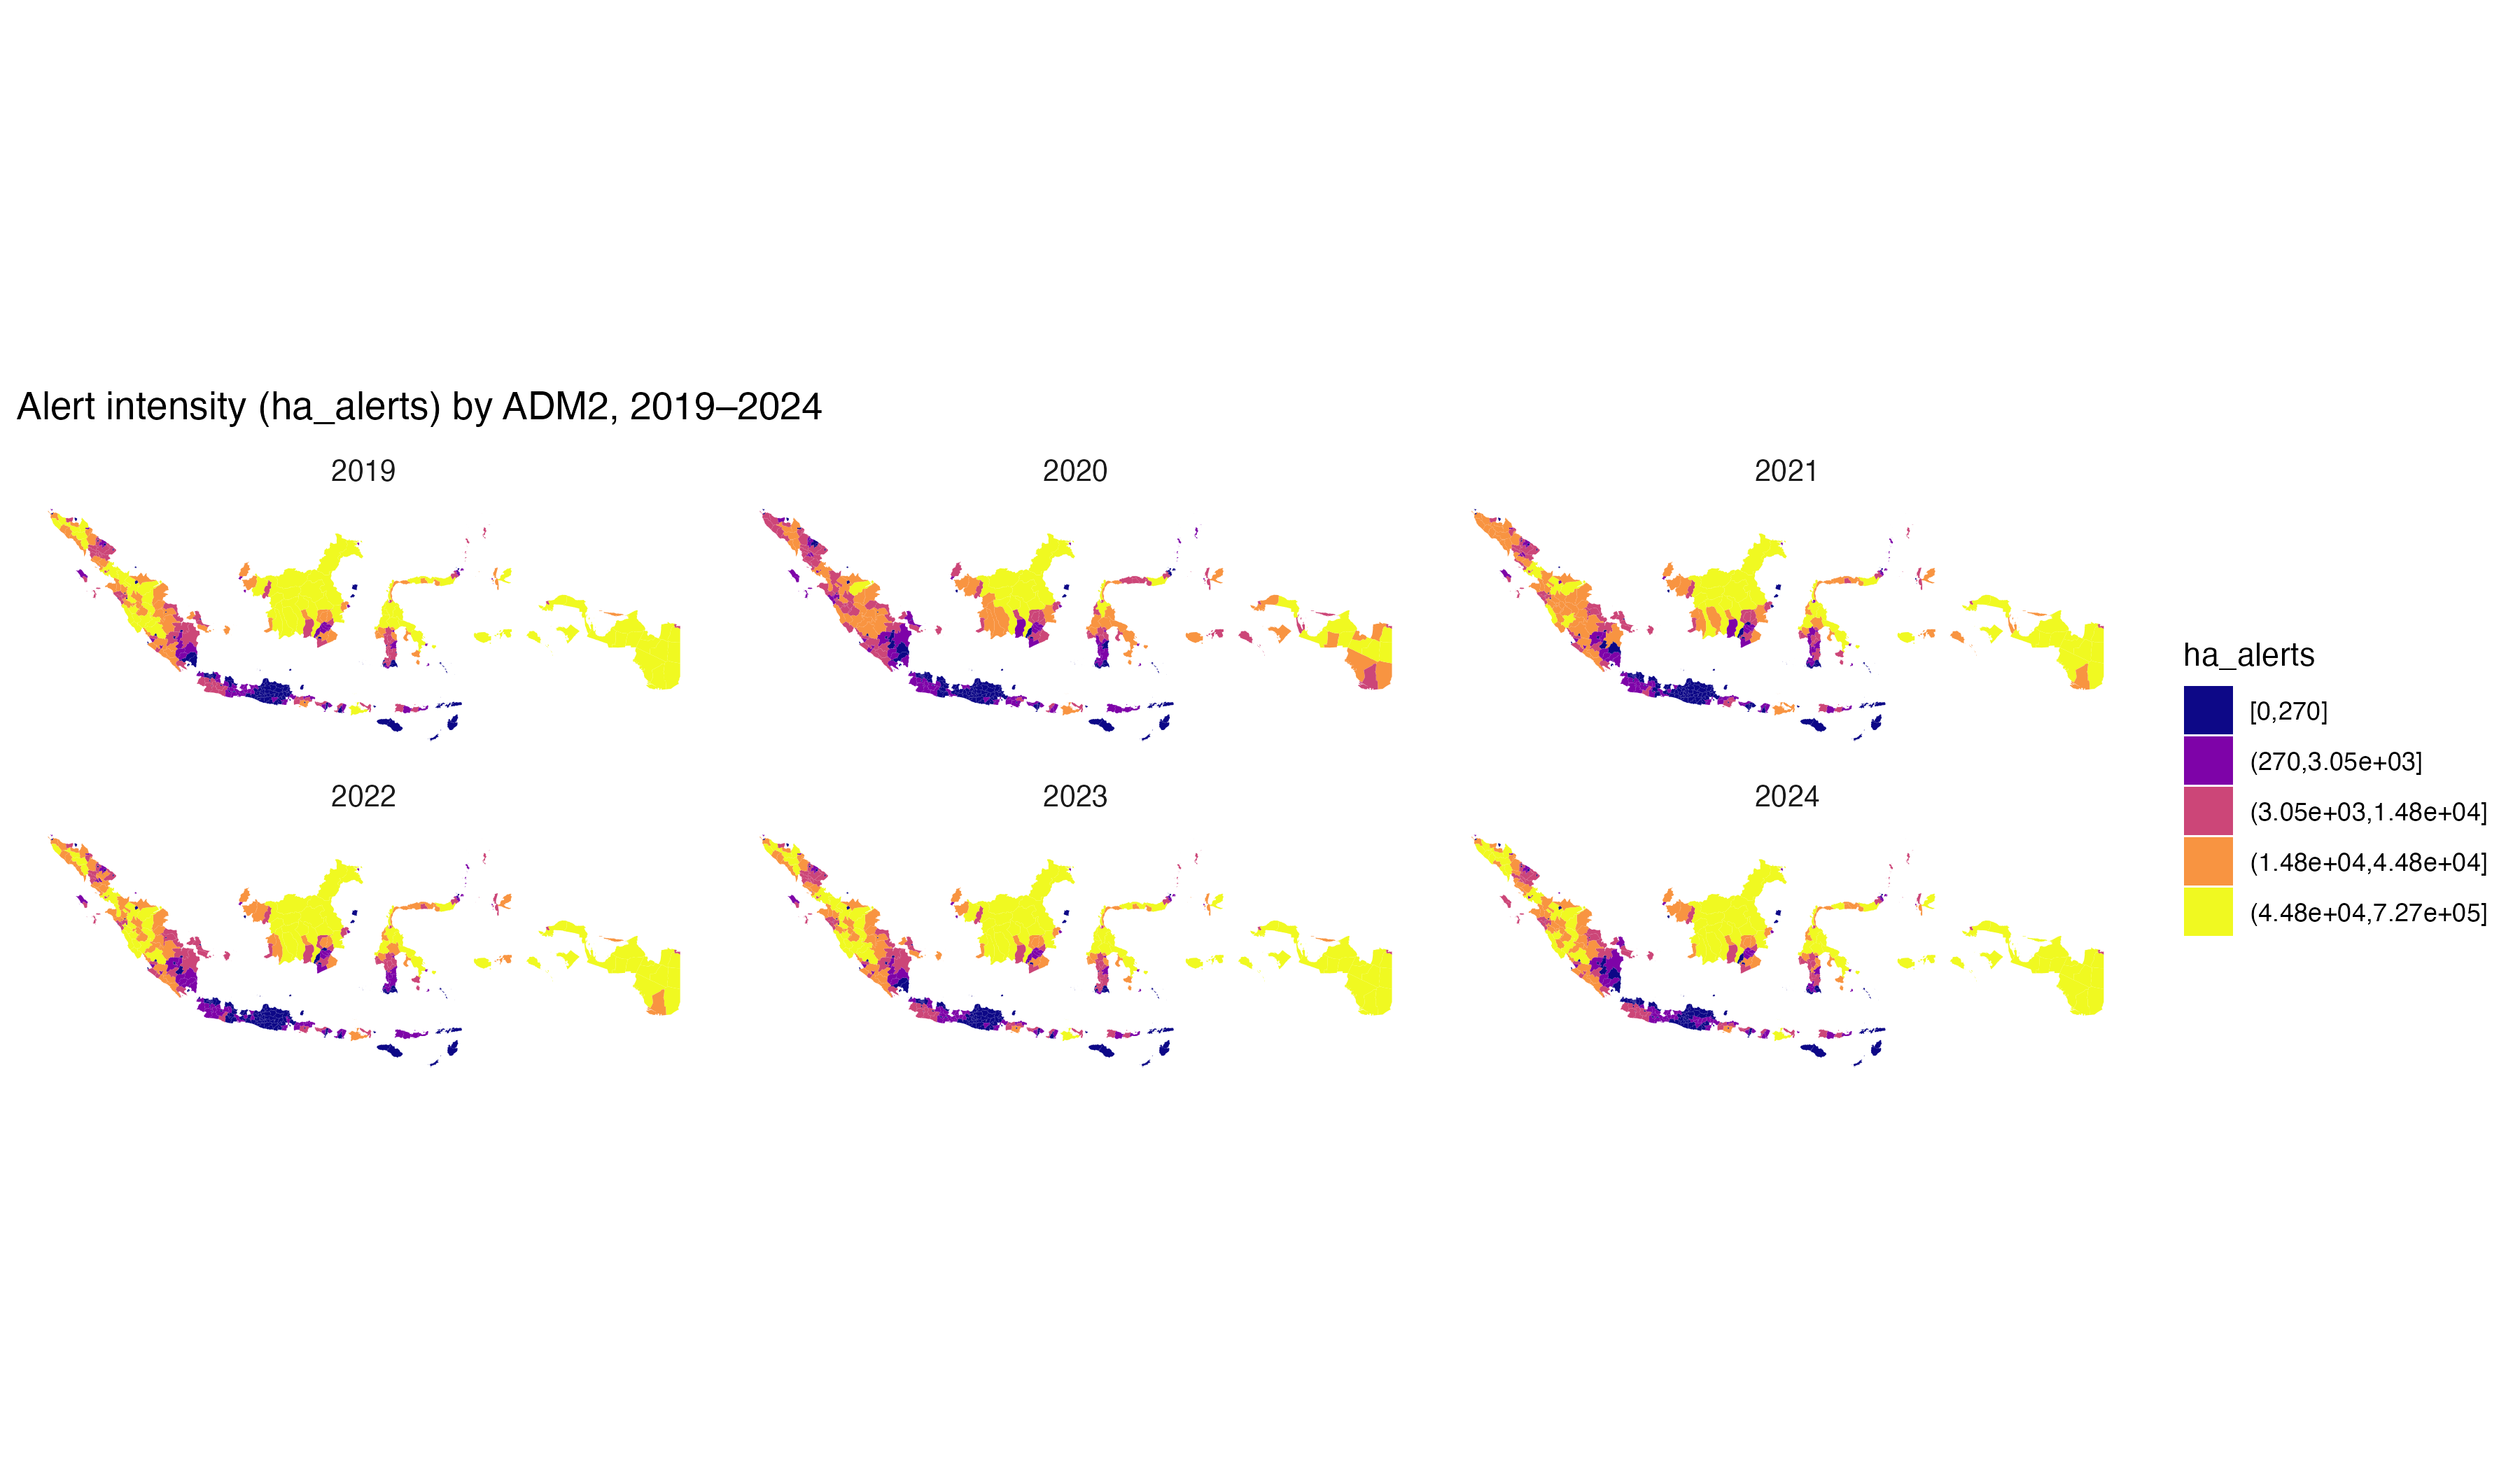
\includegraphics[width=400pt]{figures/choropleth/alerts_intensity_adm2_2019_2024.png}
  \caption{Integrated Alerts Intensity (ADM2, 2019--2024)}
  \label{fig:alerts_map}
\end{figure}

\begin{figure}[!htbp]\centering
  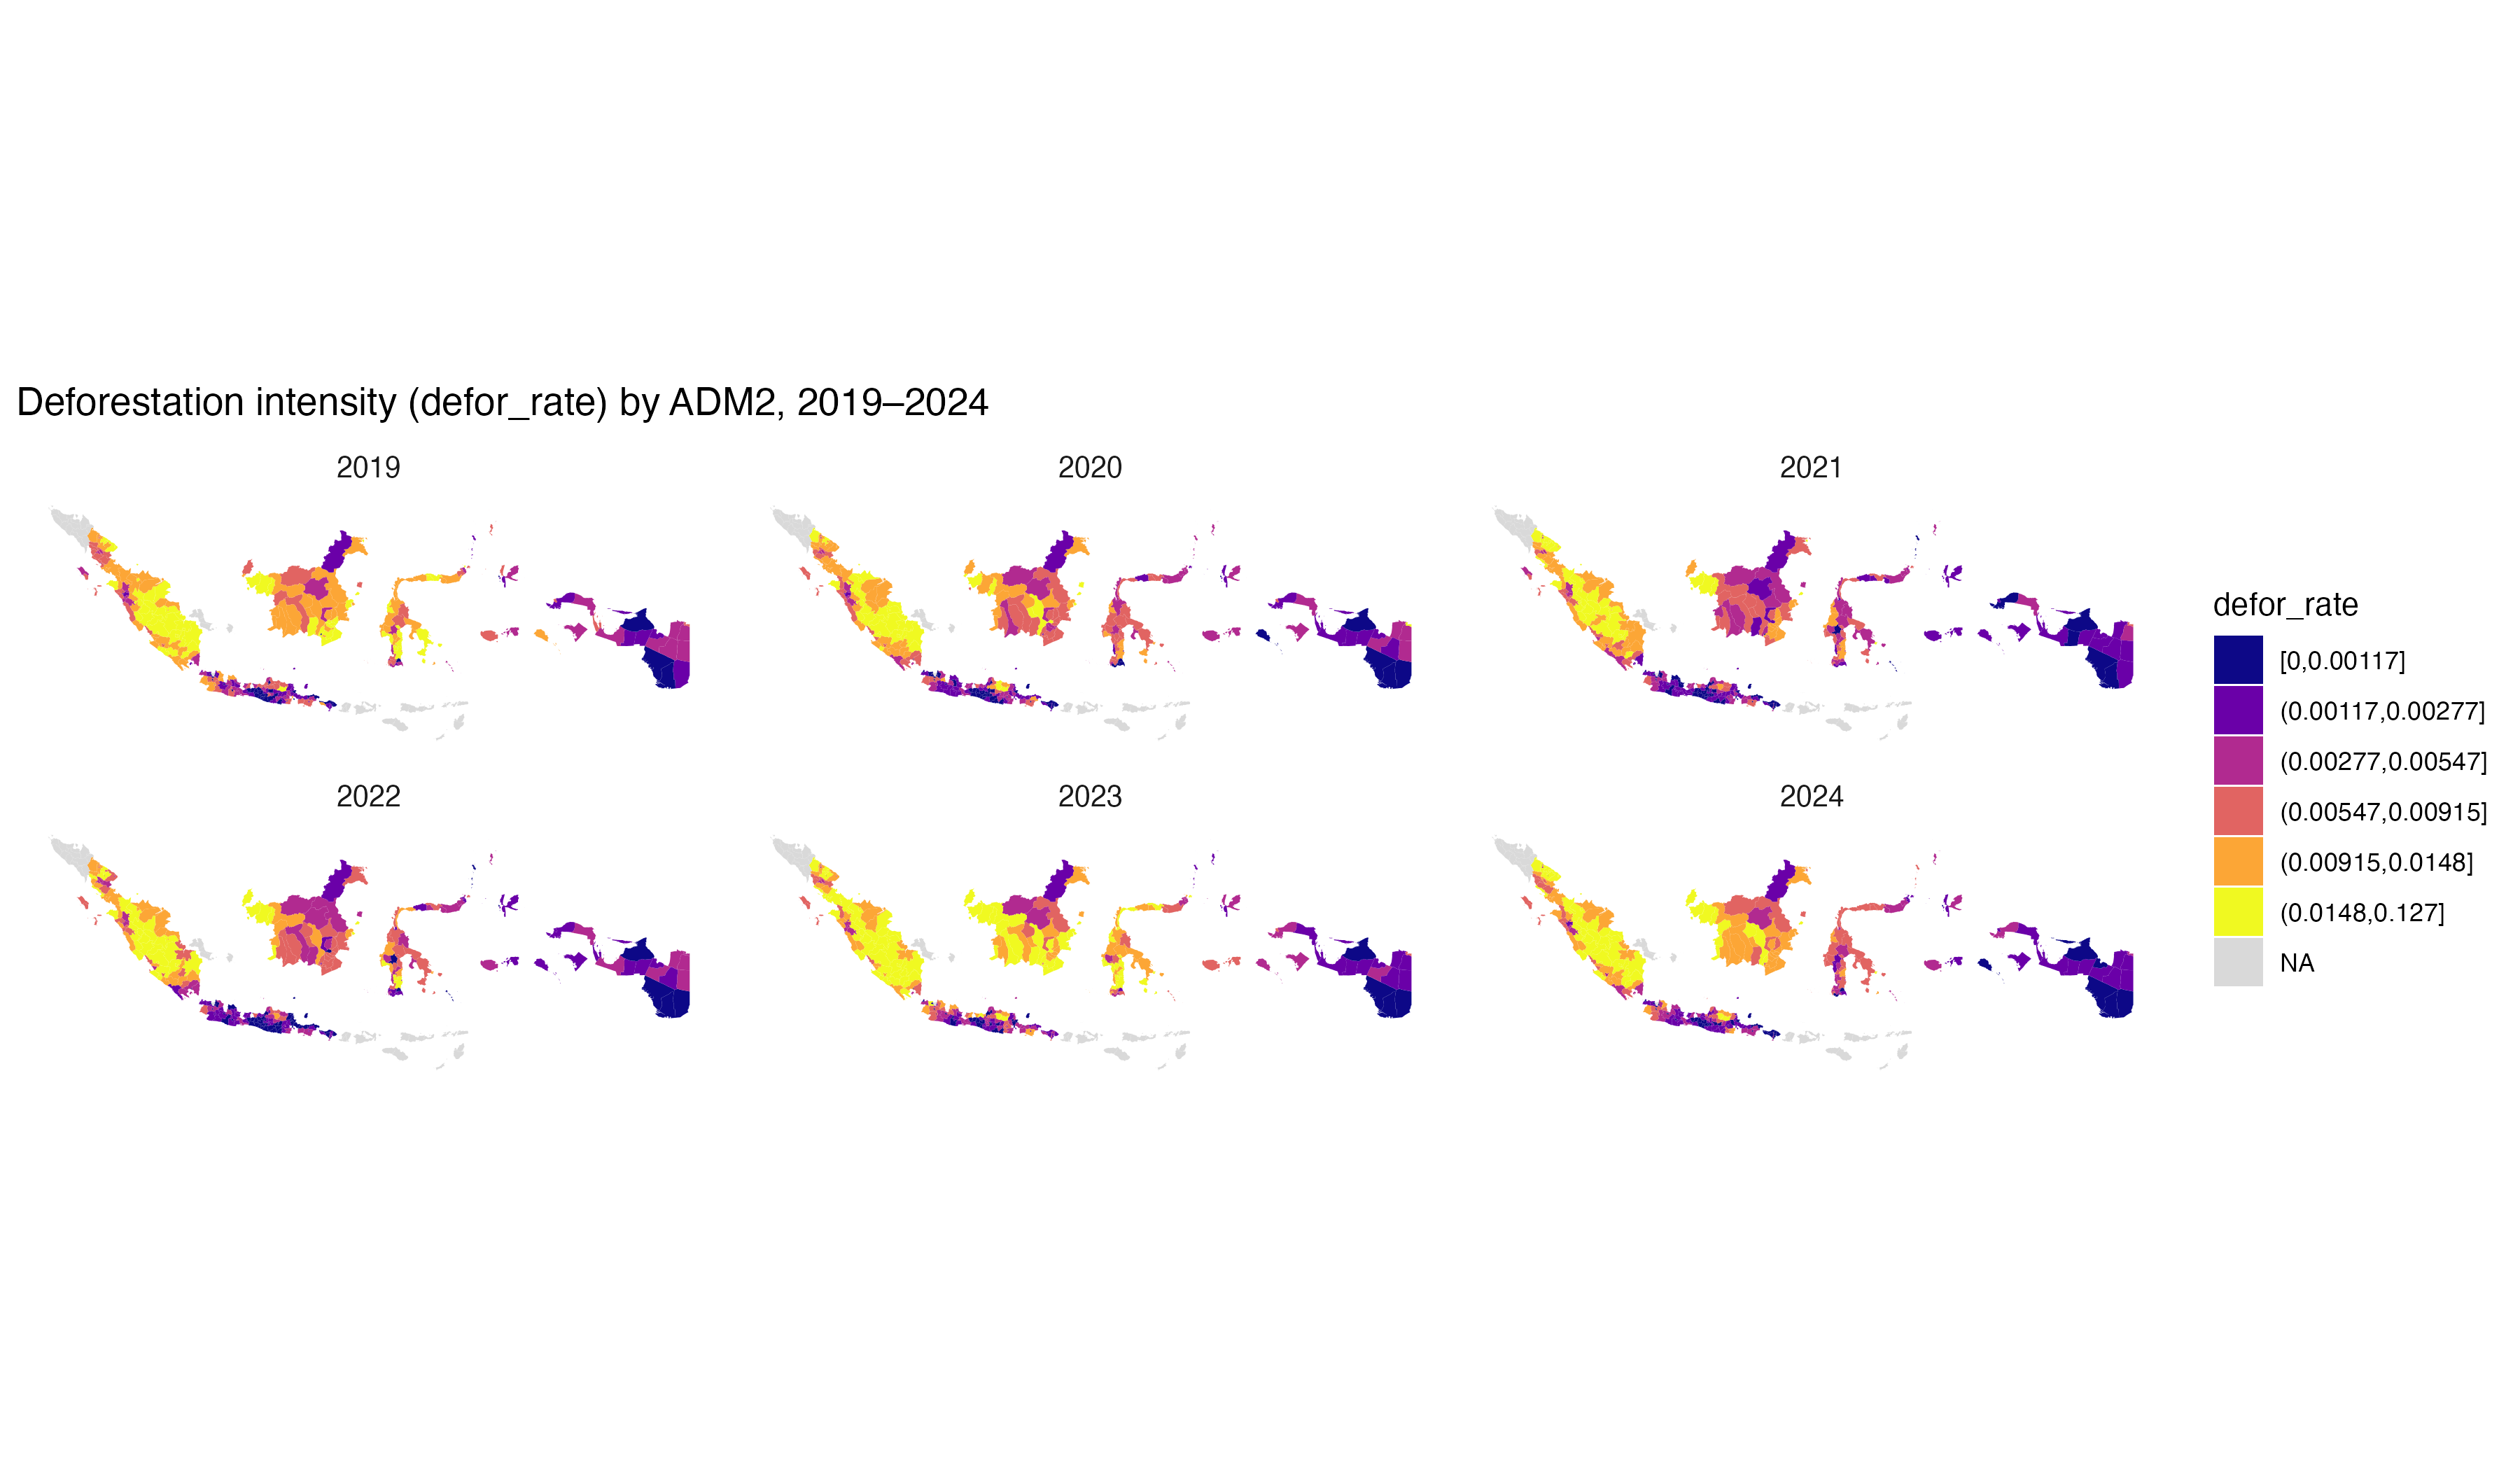
\includegraphics[width=400pt]{figures/choropleth/defor_intensity_adm2_2019_2024.png}
  \caption{Deforestation Intensity (ADM2, 2019--2024)}
  \label{fig:defor_map}
\end{figure}


%%%%%%%%%%%%%%%%%%%%%%%%%%%%%%%%%%%%%%%%
\FloatBarrier
\subsection{Histograms}

\begin{figure}[!htbp]\centering

  % 1行目
  \begin{minipage}{0.49\textwidth}\centering
    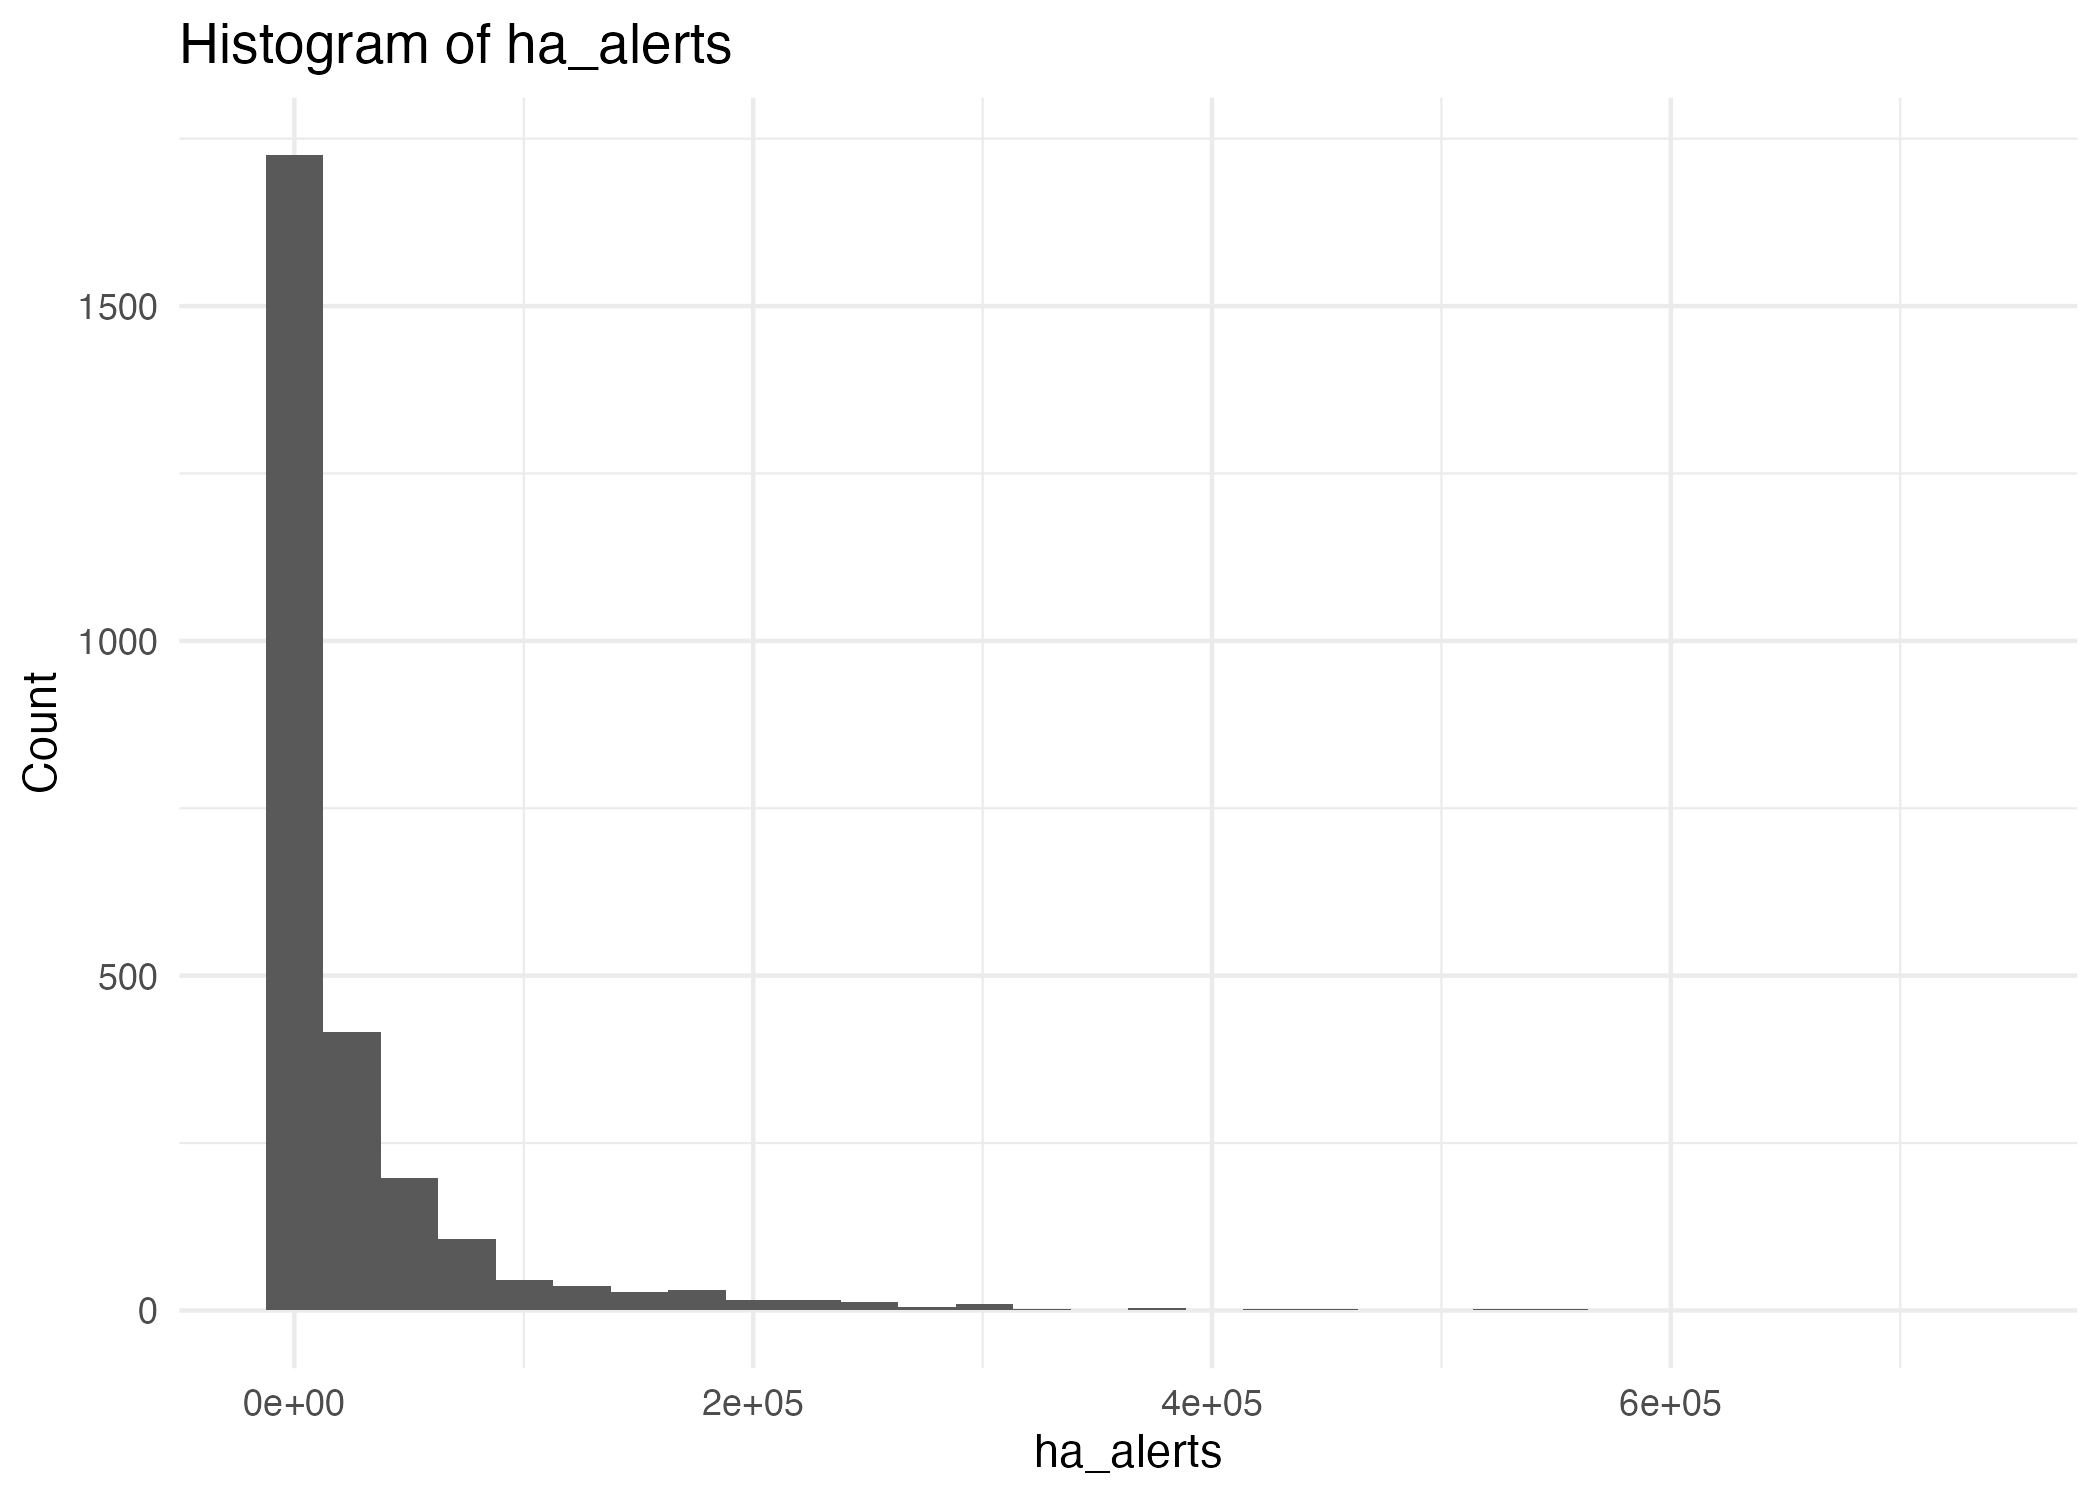
\includegraphics[width=\textwidth]{figures/hist/ha_alerts_hist.png}
    \caption*{(a) Alerts (ha)}
  \end{minipage}\hfill
  \begin{minipage}{0.49\textwidth}\centering
    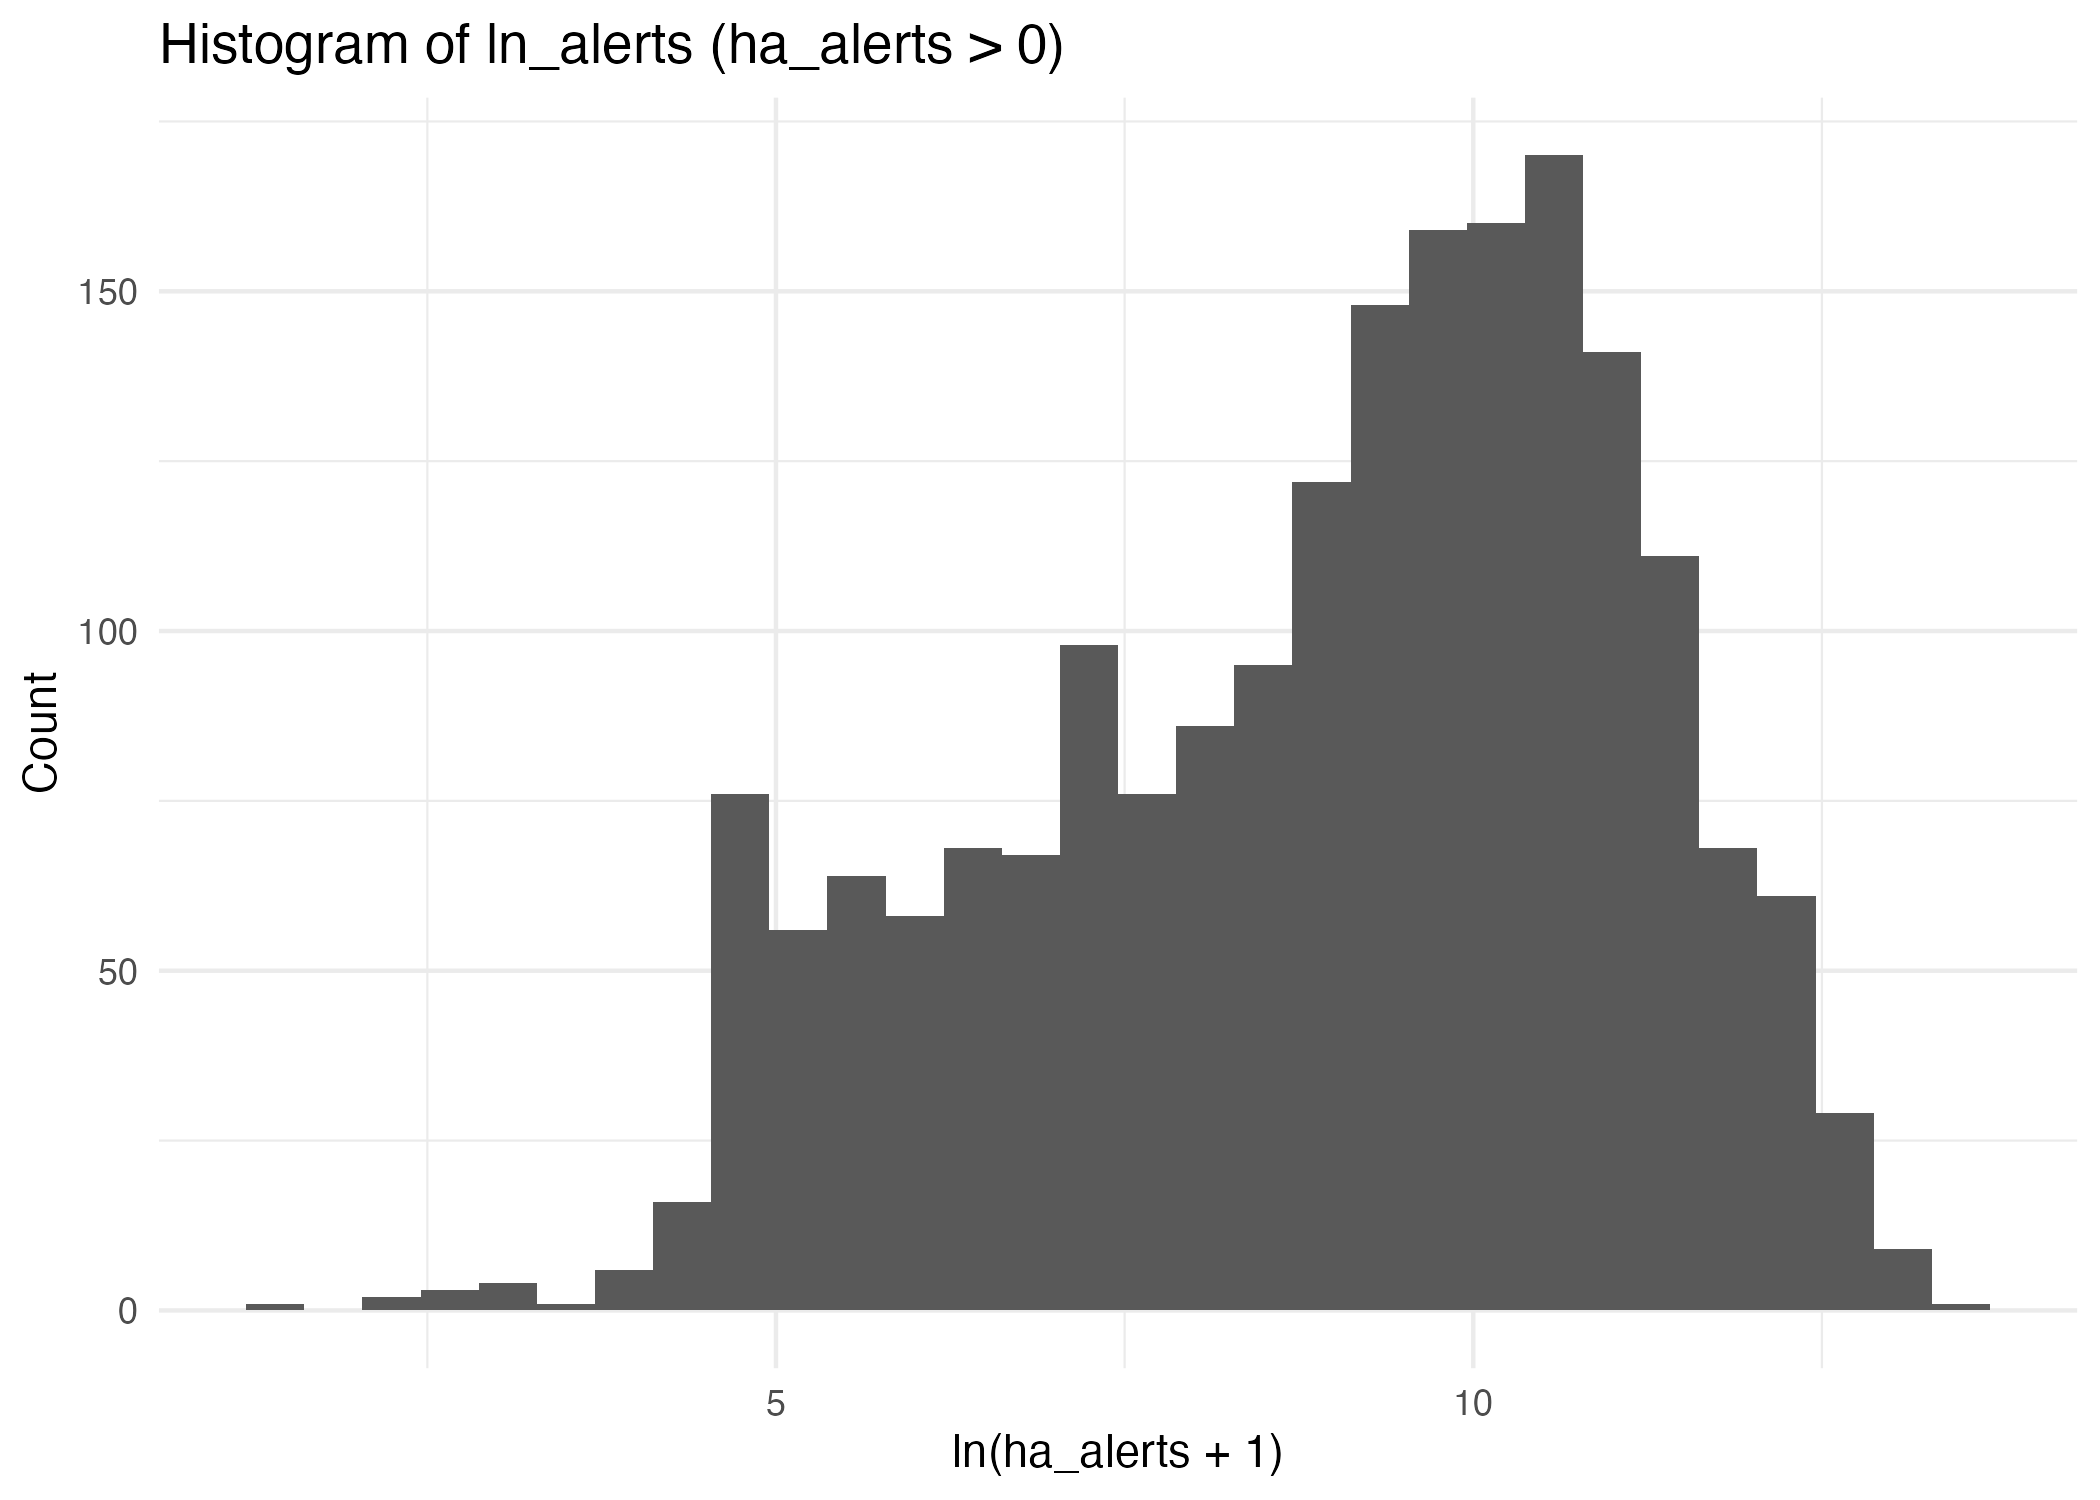
\includegraphics[width=\textwidth]{figures/hist/ln_alerts_hist.png}
    \caption*{(b) $\ln(\text{ha\_alerts}+1)$}
  \end{minipage}

  \vspace{0.6em}

  % 2行目
  \begin{minipage}{0.49\textwidth}\centering
    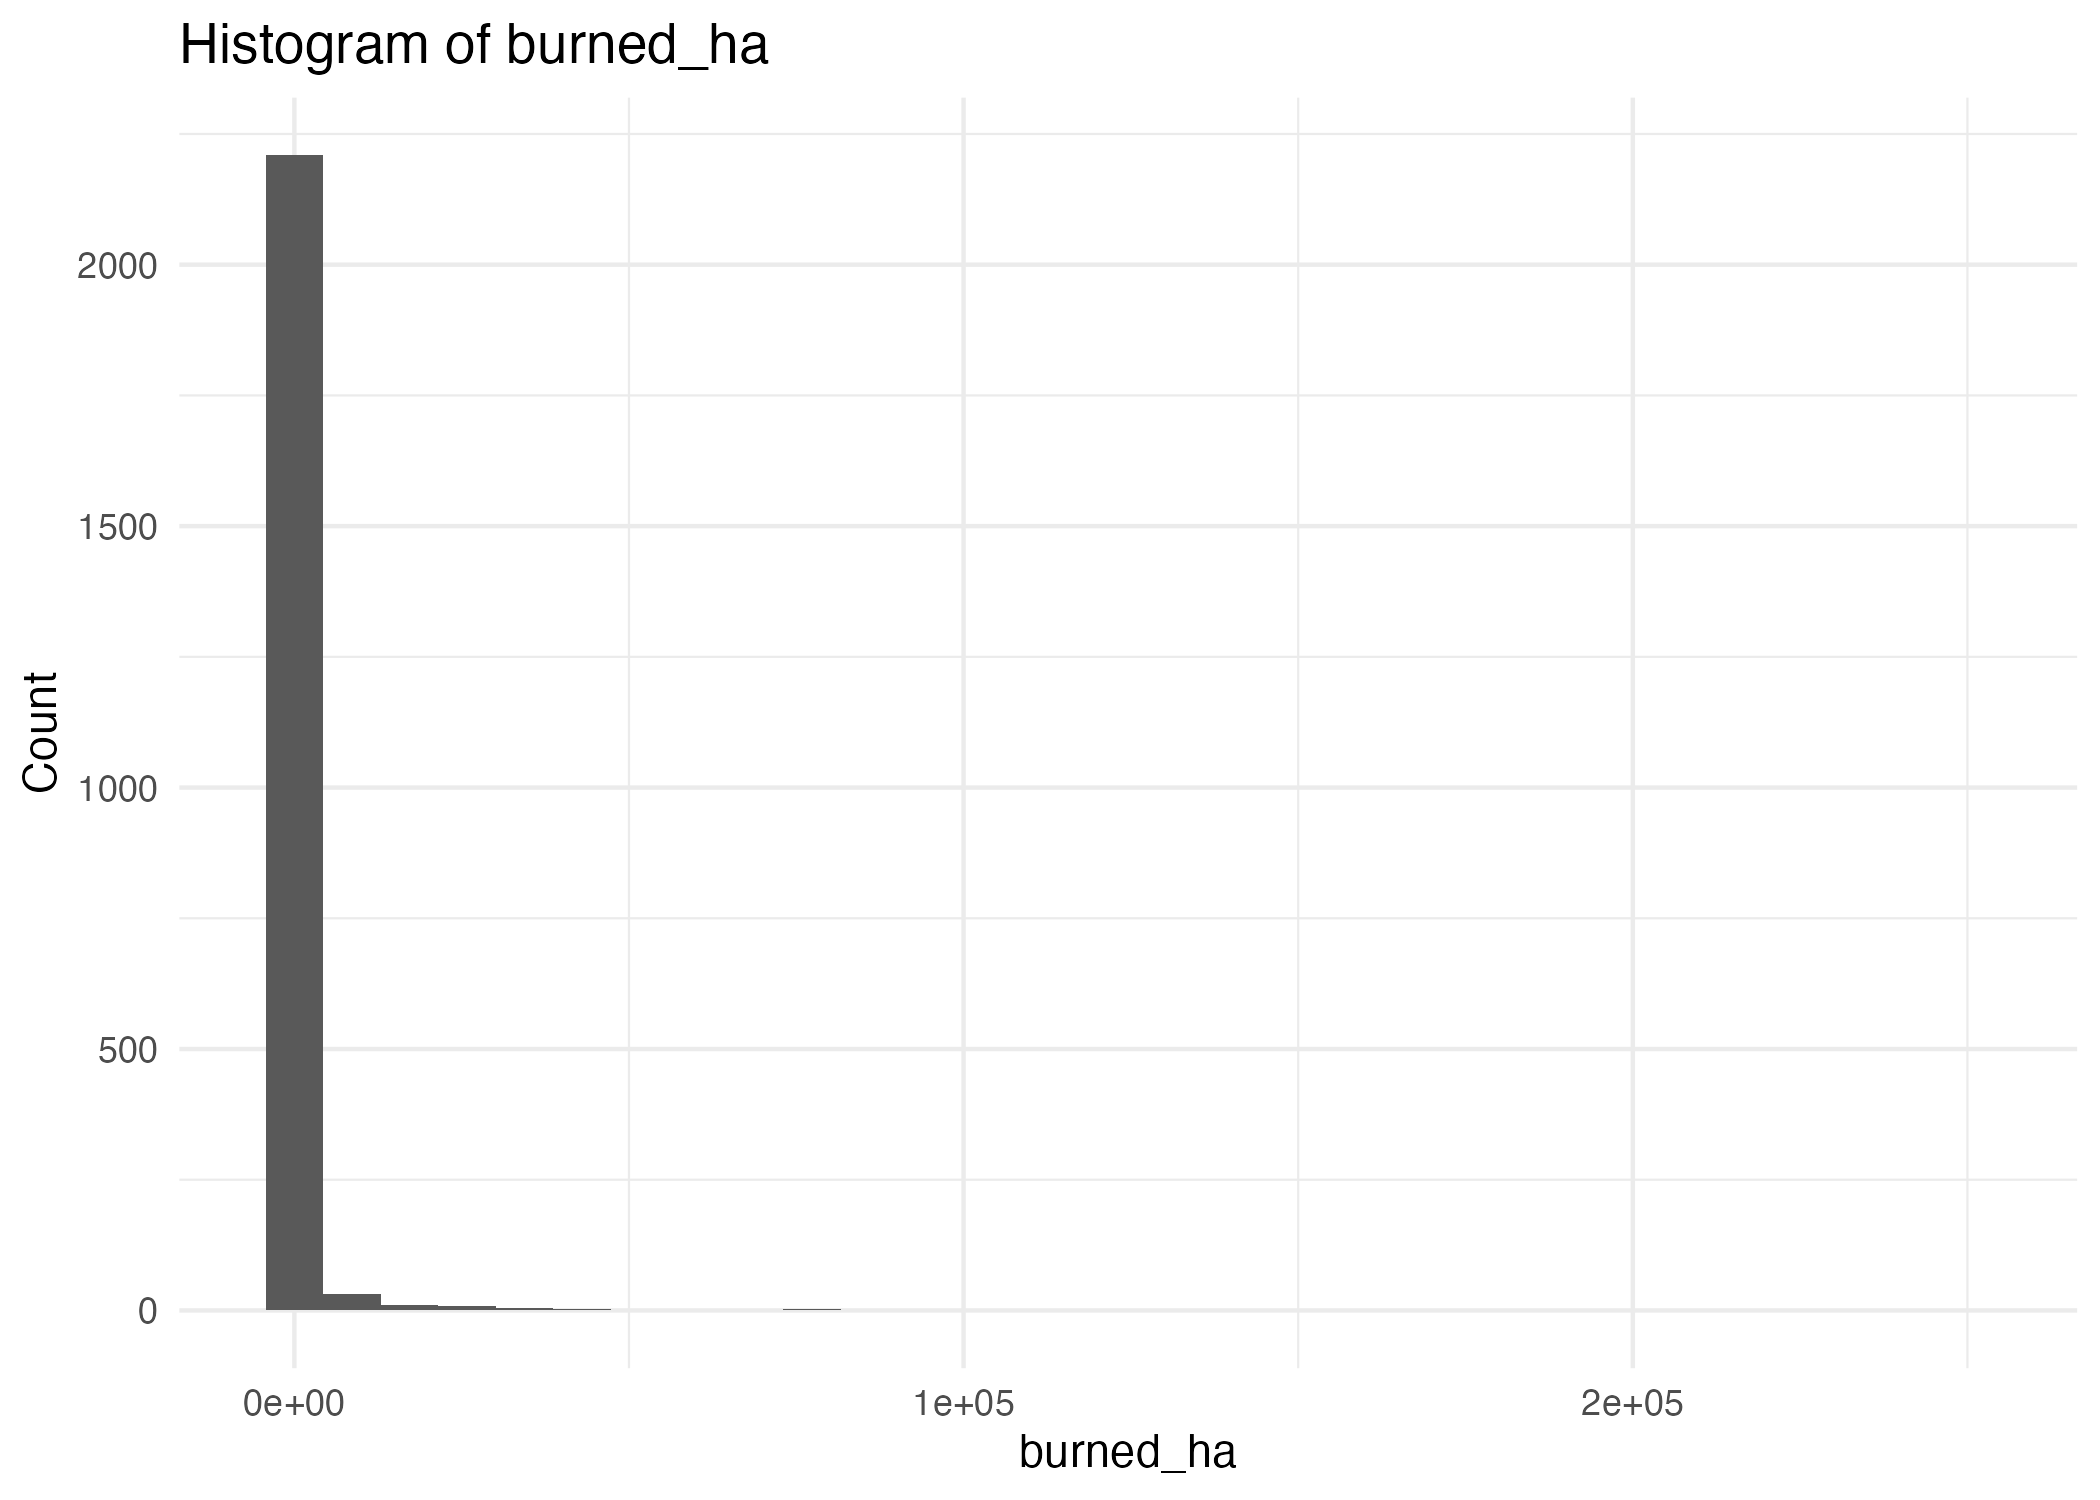
\includegraphics[width=\textwidth]{figures/hist/burned_ha_hist.png}
    \caption*{(c) Burned area (ha)}
  \end{minipage}\hfill
  \begin{minipage}{0.49\textwidth}\centering
    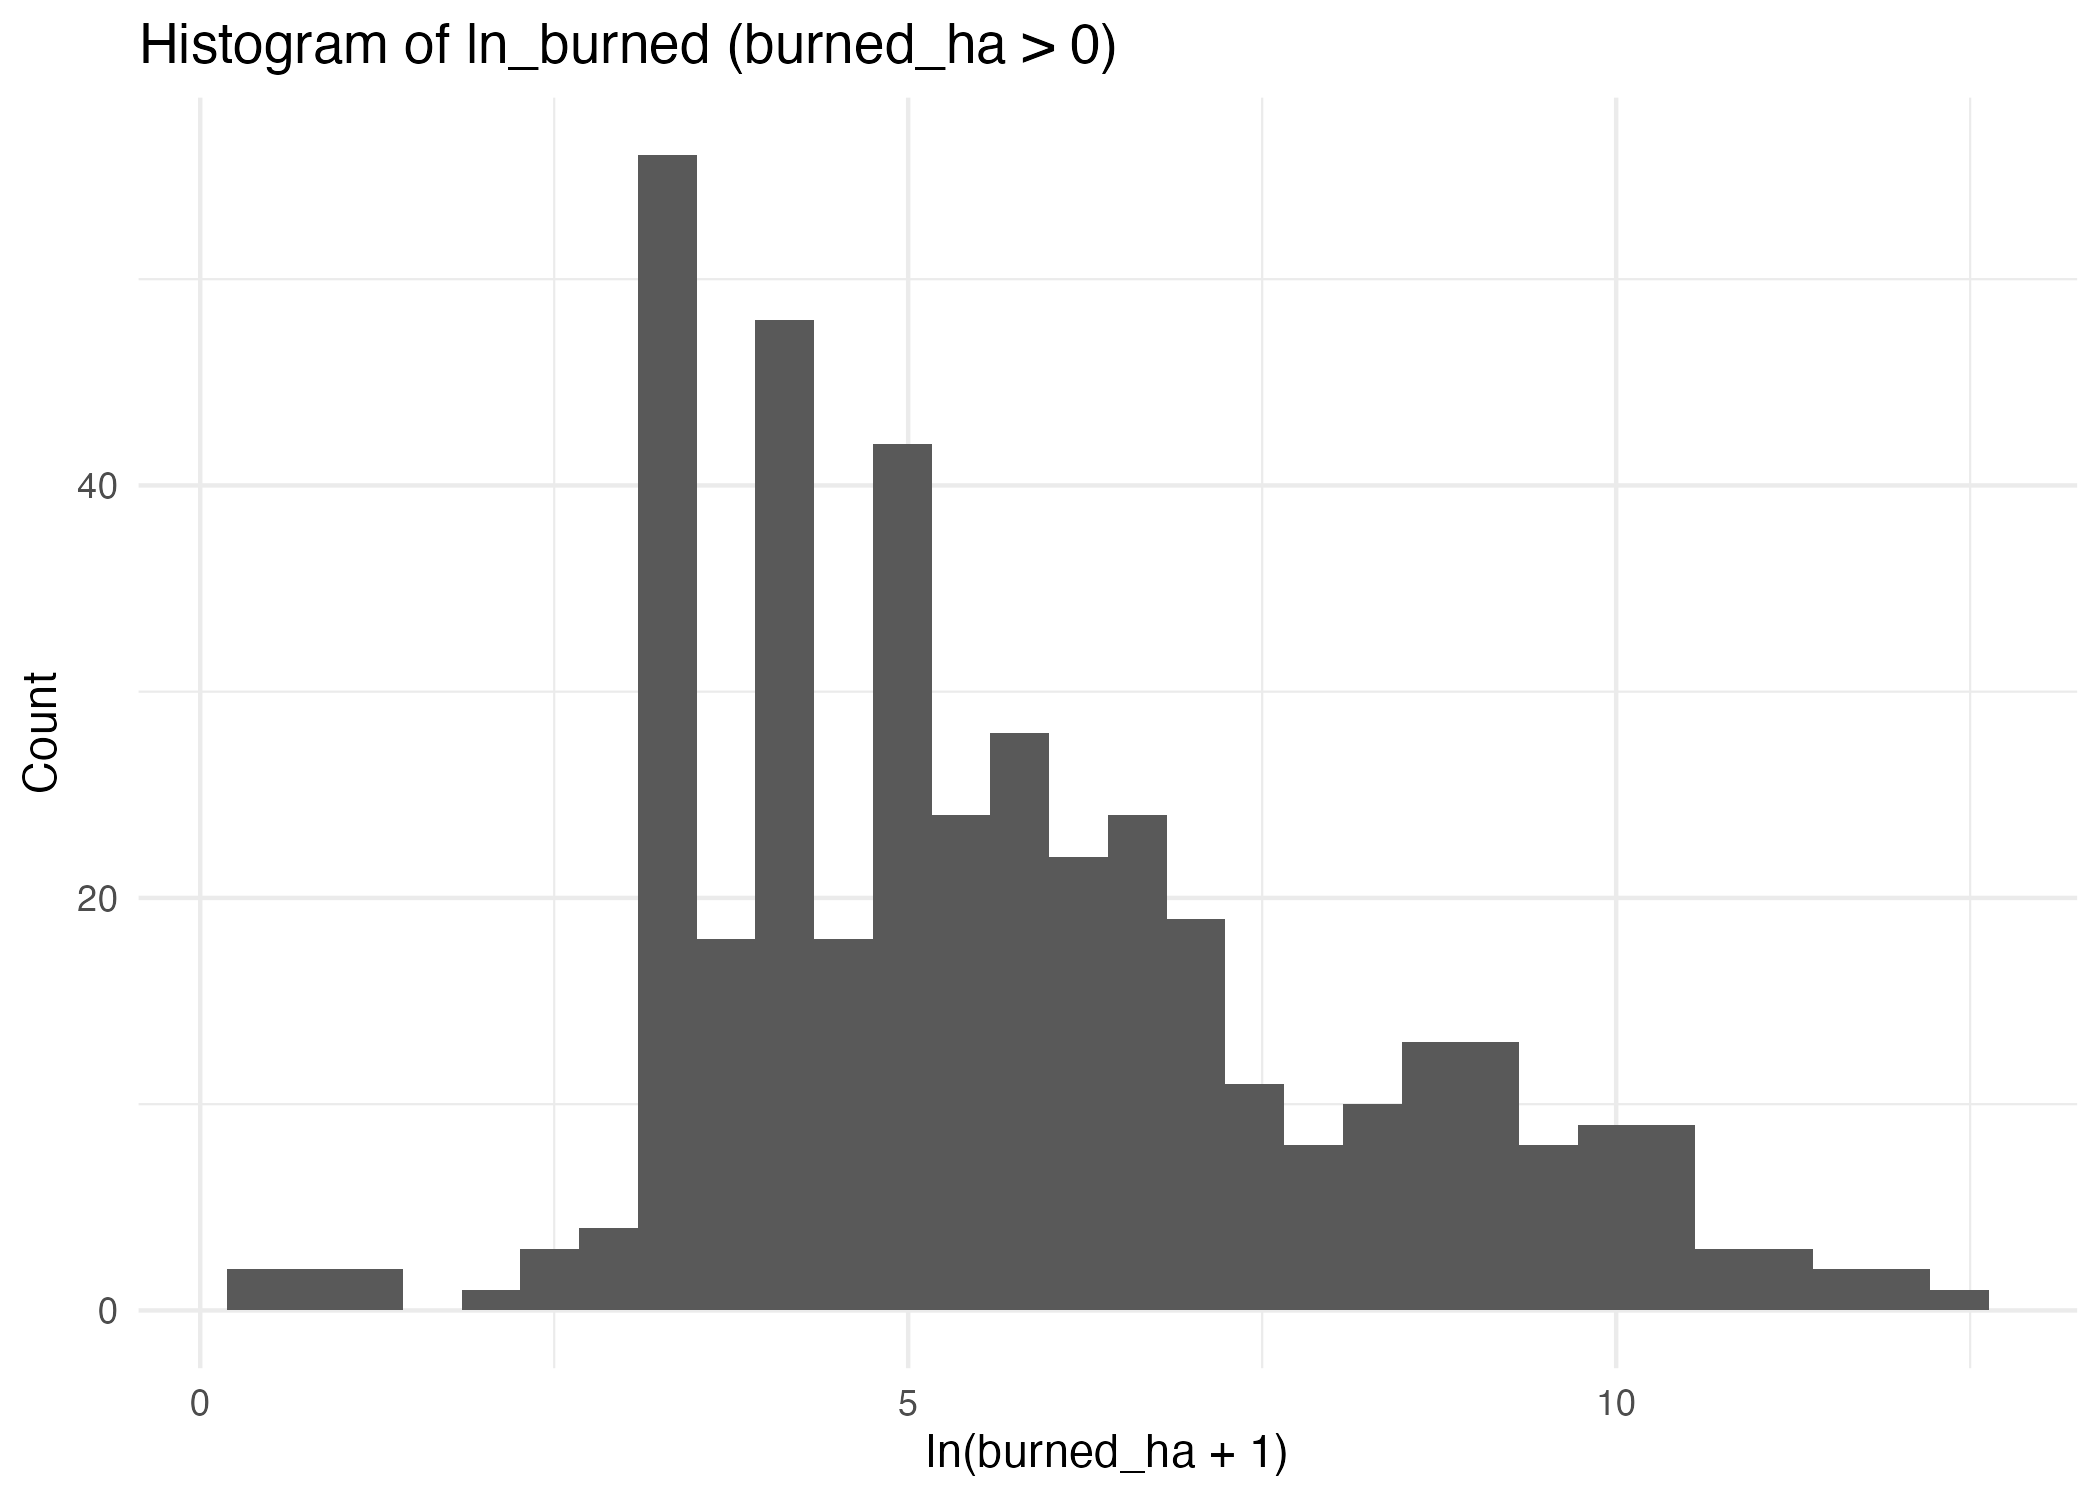
\includegraphics[width=\textwidth]{figures/hist/ln_burned_hist.png}
    \caption*{(d) $\ln(\text{burned}+1)$}
  \end{minipage}

  \caption{Histograms of key variables.}
  \label{fig:appendix_hists}

\end{figure}

%%%%%%%%%%%%%%%%%%%%%%%%%%%%%%%%%%%%%%%%
\newpage
\subsection{Scatterplots}
\begin{figure}[!htbp]\centering
  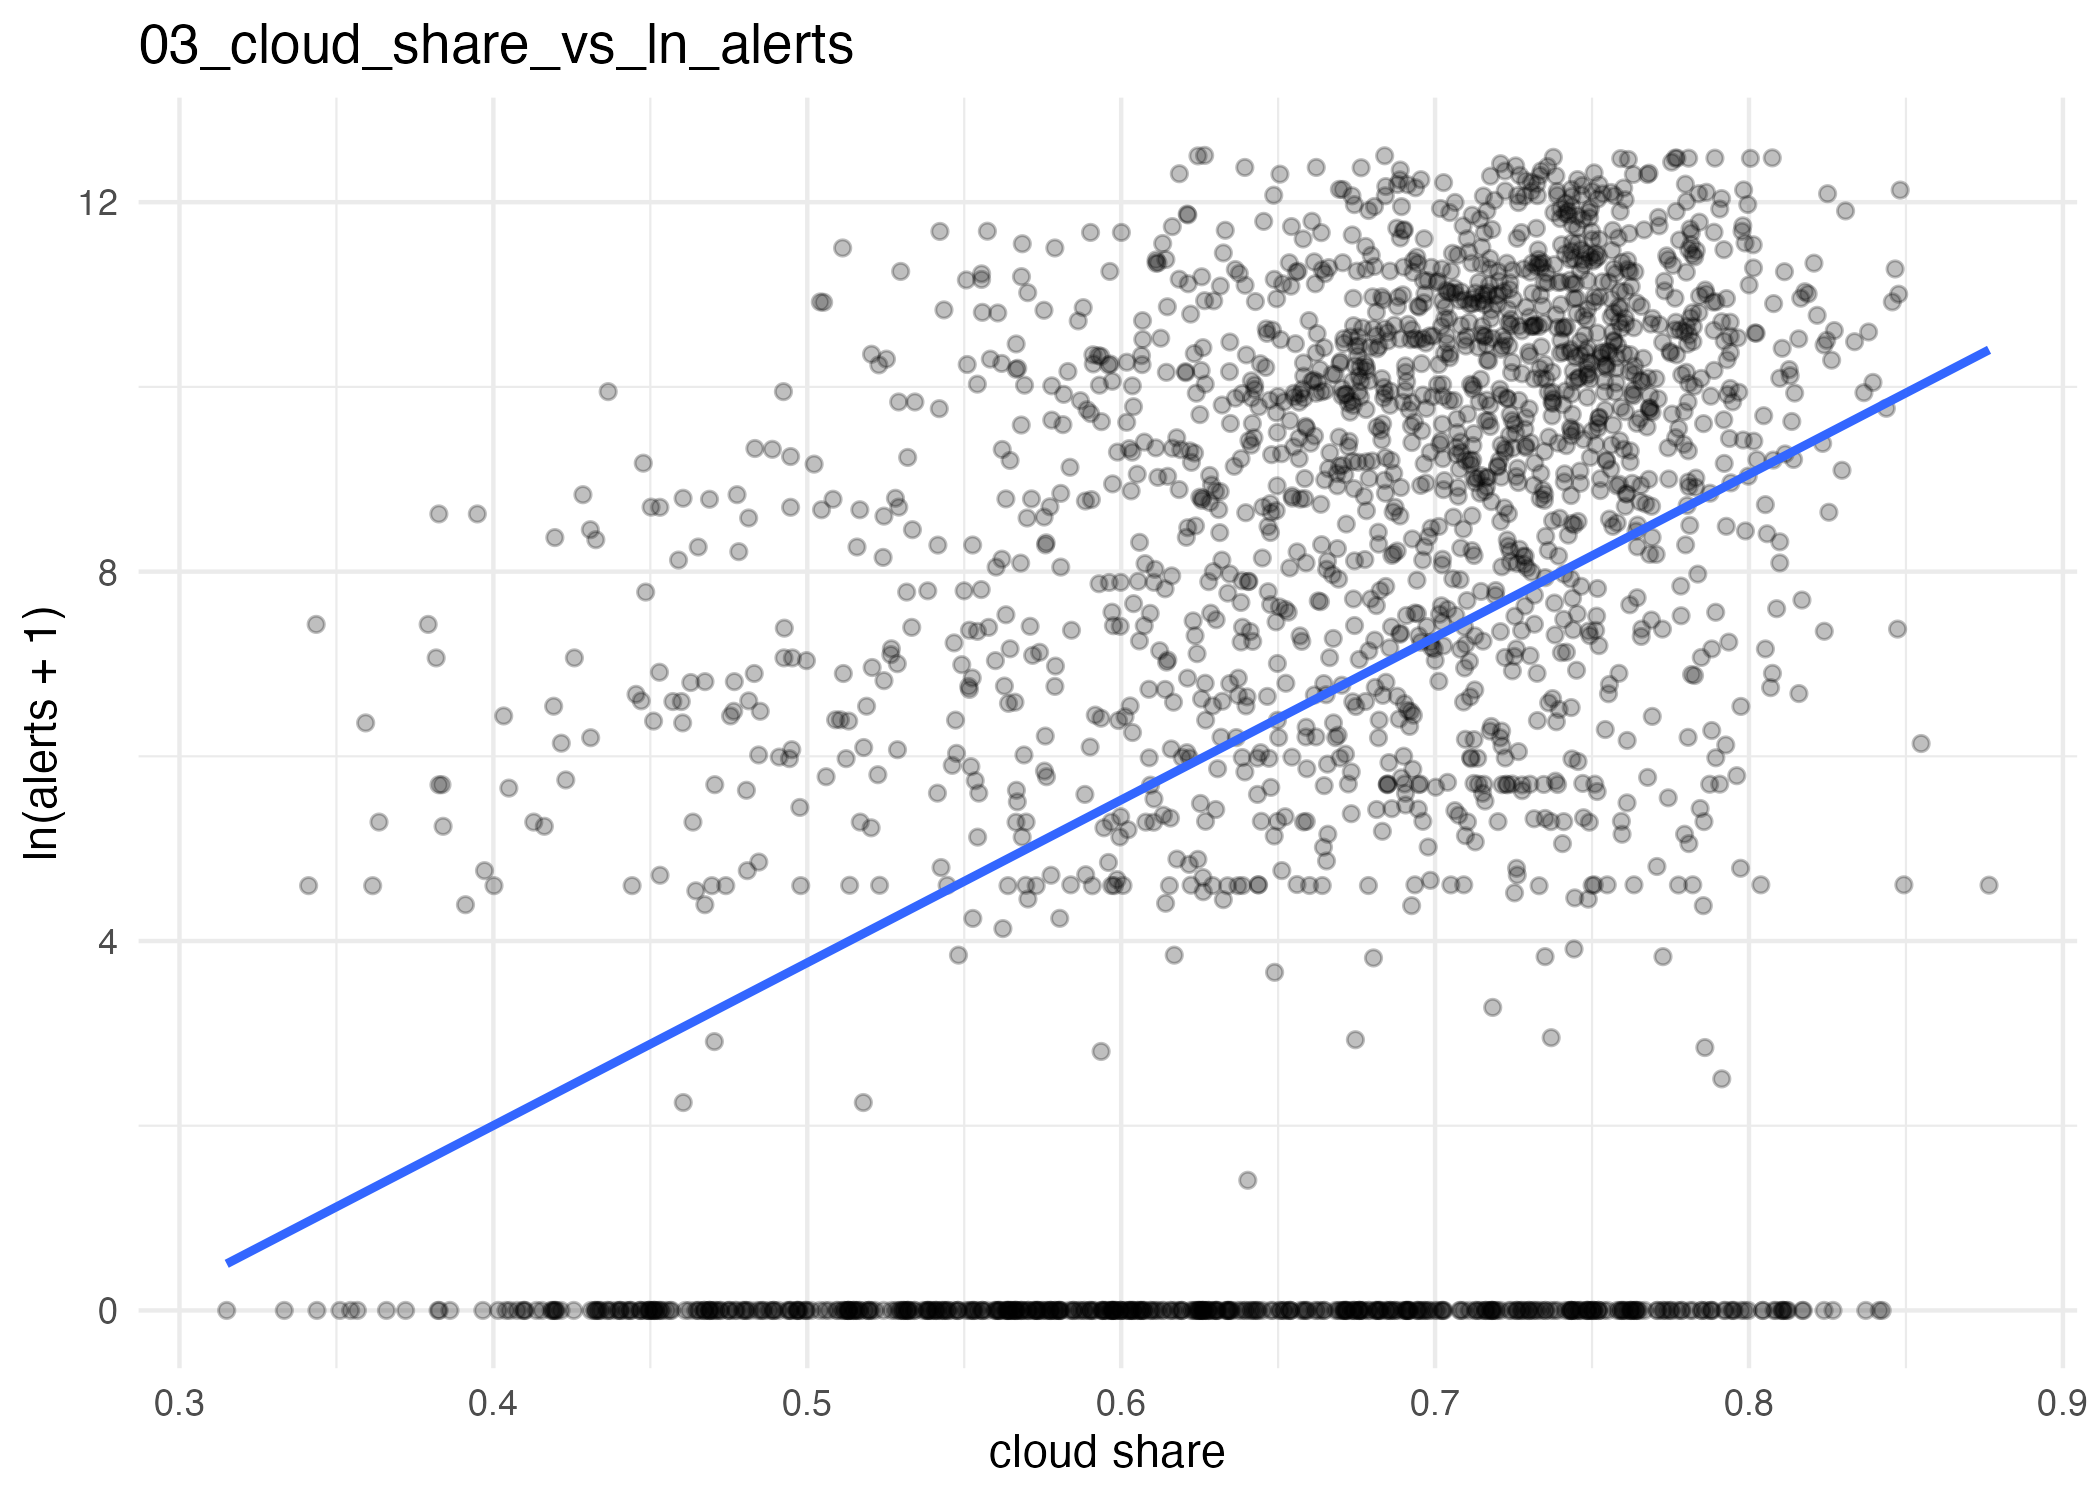
\includegraphics[width=\textwidth]{figures/scatter/03_cloud_share_vs_ln_alerts.png}
  \caption{Cloud Share vs ln Alerts}
  \label{fig:cloud_share_alerts}
\end{figure}




%%%%%%%%%%%%%%%%%%%%%%%%%%%%%%%%%%%%%%%%%%%%%%%%%%
\clearpage

%\nocite{*}

\bibliographystyle{apalike} 
\bibliography{bib/references}


\end{document}
